% !TeX program = xelatex
% !TeX encoding = UTF-8
\documentclass[final,5p,times,twocolumn]{elsarticle}

\usepackage{amsmath,amssymb,mathtools}
\usepackage{booktabs,array,multirow}
\newcolumntype{C}[1]{>{\centering\arraybackslash}m{#1}}
\usepackage{graphicx}
\usepackage{enumitem}
\usepackage{placeins}
\usepackage{dblfloatfix}
\usepackage{flafter}
\usepackage[expansion=false]{microtype}
\usepackage{xurl}
\usepackage{xcolor}
\definecolor{JMSCiteBlue}{HTML}{0072B2}
\usepackage[colorlinks=true,citecolor=JMSCiteBlue,linkcolor=JMSCiteBlue,urlcolor=JMSCiteBlue]{hyperref}
\graphicspath{{figures/}}
\setlength{\emergencystretch}{3em}
\setcounter{topnumber}{2}
\setcounter{dbltopnumber}{1}
\setcounter{dblbotnumber}{1}
\renewcommand{\topfraction}{0.90}
\renewcommand{\dbltopfraction}{0.72}
\renewcommand{\textfraction}{0.10}
\renewcommand{\floatpagefraction}{0.90}
\renewcommand{\dblfloatpagefraction}{0.95}

\journal{Journal of Manufacturing Systems}
\biboptions{sort&compress}

\newcommand{\method}{RDMCT-HBS}
\newcommand{\cmax}{C_{\max}}
\newcommand{\pdi}{\mathrm{PDI}}
\newcounter{algorithm}
\newcommand{\algorithmtitle}[1]{\refstepcounter{algorithm}\noindent\textbf{Algorithm~\thealgorithm: #1}\par\smallskip}

\begin{document}
\begin{frontmatter}

\title{An operational decision framework for dual-source mixed-flow PECVD rotating-chamber cluster tools}

\author[ustb]{Lizhen Shao\corref{cor1}}
\ead{lshao@ustb.edu.cn}
\author[ustb]{Lincong Wei}
\ead{m202420836@xs.ustb.edu.cn}
\author[ustb]{Wei Wang}
\cortext[cor1]{Corresponding author.}
\address[ustb]{Department of Control Science and Engineering, University of
Science and Technology Beijing, No. 30 Xueyuan Road, Haidian District,
Beijing 100083, China}

\begin{abstract}
This study develops an operational decision framework for PECVD rotating-chamber cluster tools supplied by product wafers from the atmospheric side and reusable dummy wafers from vacuum-side storage. The two material flows share robots and multi-position chambers, coupling material availability, full occupancy, processing, and periodic cleaning. A two-stage mixed-integer linear programming model represents two processing modes and the complete routes of both wafer types. Structure-based initial schedules and learning-enhanced cut selection support time-limited solution search. Computational experiments show that, under prescribed PW layouts, the preferred mode depends on lot size, cleaning interval, and complete-chain segmentation. For a 16-wafer configuration without cleaning, chained processing reduces makespan by 4.87\% relative to parallel processing. The two-stage workflow improves waiting and processing cadence, while precomputed structured initial schedules increase feasible-schedule availability during the subsequent timed solve. The framework provides a consistent basis for mode selection, dummy-wafer allocation, and event scheduling in dual-source mixed-flow equipment.
\end{abstract}

\begin{keyword}
semiconductor manufacturing system \sep cluster tool \sep dual-source material flow \sep
operational decision \sep mixed-integer linear programming \sep learning-enhanced exact optimization
\end{keyword}

\end{frontmatter}
\section{Introduction}
\label{sec:intro-new}

Three-dimensional device structures and multilayer thin-film integration impose increasing demands on deposition uniformity, processing capability, and equipment output per unit floor area \citep{appliedprecisioncvd}. Plasma-enhanced chemical vapor deposition (PECVD) is an important thin-film deposition process. Cluster tools (CTs) integrate process modules, vacuum-handling robots, and load locks so that wafers can be loaded, processed, and returned within a controlled environment. Tool output depends on coordination between processing and handling; load-lock switching, chamber cleaning, and residency limits further constrain feasible operation \citep{pan2018survey}.

Multi-space process modules and multi-finger robots provide a structural basis for parallel processing within an equipment cell \citep{gu2024applied,gu2024multifinger}. This study considers a four-position rotating-chamber CT for PECVD. Rotation changes the positions accessible to the robot and connects multi-wafer processing with paired handling. In this configuration, PECVD specifies the process and recipe durations, while chamber rotation enables position changes and transitions between consecutive processing cycles. Their combination determines processing organization and loading and unloading order.

The tool uses product wafers and reusable dummy wafers. Product wafers initially occupy atmospheric-side load ports and enter the vacuum domain through the atmospheric transfer robot (ATR), aligner (AL), and load locks (LLs). Dummy wafers are preloaded in a storage unit mounted in the vacuum domain and are accessed directly by the vacuum transfer robot (VTR). We call this supply structure dual-source. Under the full-occupancy recipe considered here, dummies fill positions not occupied by products and provide the occupancy required for cleaning. Their inventory and reuse times therefore constrain subsequent product processing.

The two wafer types have different origins and circulation routes but share the VTR and rotating-chamber positions, forming mixed-flow operation (Fig.~\ref{fig:system-en-new}). Product flow connects atmospheric-side batch input to processed-wafer return; dummy flow circulates between vacuum storage and the chambers. Full occupancy, dummy inventory, and shared-resource timing couple these routes. Admission of a product wafer pair thus depends jointly on product arrival, dummy availability, chamber state, and robot position. Scheduling must represent the supply, convergence, and return of both material flows.

Two preset modes are considered: $4\times1$ parallel processing and $2\times2$ chained processing. The former processes four wafers synchronously in one exposure. The latter uses wafer pairs (PWs) as handling and occupancy units, alternating loading and unloading between adjacent cycles so that each product wafer participates in two consecutive exposures. Conditional on both recipes meeting the relevant product-process requirements, the comparison holds cumulative nominal processing time per wafer constant. Differences in cycle count, occupancy, and exchange order produce different cleaning positions and dummy demands for the same lot. Cleaning occupies chambers and changes return times, thereby affecting subsequent chain transitions. The resulting decision problem coordinates modes, dual-source material flow, and equipment actions under residency and capacity constraints to shorten finite-batch makespan and improve waiting and processing cadence.

\begin{figure}[t]
\centering
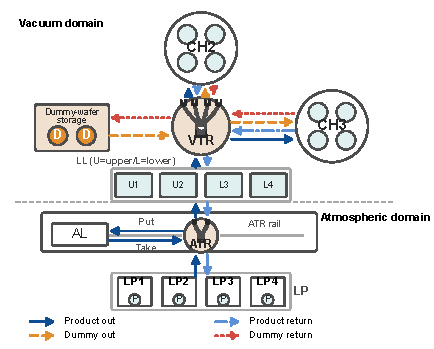
\includegraphics[width=\linewidth]{fig_system_en_nature}
\caption{Dual-source mixed-flow rotating-chamber CT. Products enter the vacuum domain from atmospheric-side LPs through ATR, AL, and LLs; dummies enter from vacuum storage through VTR. Solid, dash-dot, dashed, and dotted arrows indicate product outbound, product return, dummy outbound, and dummy return routes, respectively.}
\label{fig:system-en-new}
\end{figure}

Manufacturing-system research coordinates processing resources, logistics, and production data through multi-agent architectures, joint layout and scheduling, and transferable control representations \citep{li2025selforganizing,zhu2025matrix,bhatta2025scaling}. In semiconductor manufacturing, industrial data spaces and historical decision knowledge support data organization and dynamic dispatching \citep{chen2024idwfs,chen2025dgrl}, while quality constraints guide route selection, equipment allocation, and job sequencing \citep{kim2025yieldmakespan,lee2026quality}. This study addresses how production decisions are realized within an equipment cell: batch and recipe inputs must become action sequences satisfying material-supply, chamber-occupancy, and handling constraints.

CT research established analytical foundations for throughput and residency feasibility. Analytical models relate processing and handling times to throughput \citep{perkinson1994throughput}; linear programming, heuristics, and timed Petri nets produce feasible or optimal schedules under residency constraints \citep{rostami2002optimal,wu2010closedform,qiao2012sojourn}. Subsequent models address revisiting processes, multiple wafer types, and selectable process modules \citep{qiao2014revisiting,wang2020multiple,wang2025virtualcell}. Steady-state analysis of four-finger robots and four-space modules, together with joint optimization of two-type wafer releases and robot actions, provides a basis for more complex tool structures \citep{gu2024multifinger,yang2025miptwowafers}. Finite batches additionally require chain initialization, termination, and partial-batch filling, making actual dummy-supply and return times constraints on subsequent processing.

Cleaning and shared resources further couple material routes. Task-sequence enumeration, partial loading and timing control, virtual-wafer occupancy, and chamber-state-dependent triggers coordinate cleaning with production \citep{kim2013cleaning,yu2020delay,qiao2022binary,li2022conditioncleaning}. Shared-buffer synchronization and dynamic action screening address deadlock during failure shutdown and noncyclic operation \citep{zhu2025failuredeadlock,kim2025noncyclicdeadlock}. Waiting constraints also affect equipment output and upstream control \citep{lee2018waiting}. In the present configuration, cleaning changes dummy occupancy, chain segmentation, and shared-VTR service order simultaneously, requiring joint scheduling of complete product routes and closed-loop dummy routes.

Learning can select CT actions directly or support mathematical optimization. Deep reinforcement learning with look-ahead search addresses noncyclic control, while DDPG has been used to adjust PVD processing times in simulation \citep{kim2025adaptivecluster,hong2026ddpgct}. Here, recipe durations are inputs and learning is embedded in MILP cut selection. Relevant approaches include reinforcement-learning selection, cut ranking, and look-ahead imitation \citep{tang2020cut,huang2022cutranking,paulus2022looking}; HEM jointly selects cut counts and ordered sequences \citep{wang2023hem}. This hierarchical policy provides a basis for incorporating equipment-variable roles while retaining the constraint model.

This study examines the joint effects of product supply, dummy reuse, and cleaning organization. Under a prescribed mode and PW layout, dummy return times constrain subsequent full-occupancy processing, while complete chains determine the available cleaning boundaries. The model jointly converts these material dependencies and shared-resource orders into event times. The contributions are:
\begin{enumerate}[leftmargin=*]
\item A material-flow model couples atmospheric-side product supply and vacuum-side dummy reuse through full chamber occupancy, cleaning, and shared handling resources. It generates complete finite-batch event schedules for both preset processing modes.
\item A two-stage MILP first minimizes product-return makespan, then refines waiting and cadence while retaining the makespan bound and principal discrete order. Mode comparisons quantify how lot size and cleaning interval change preferred operation through complete-chain segmentation under prescribed PW layouts.
\item A structure-aware solution framework combines SPBS initialization with a role-aware hierarchical cut selector. Matched-budget experiments separately evaluate initialization, timing refinement, and cut selection, identifying their contributions to feasible-schedule availability and solution quality.
\end{enumerate}

Section~2 presents the equipment architecture, material flows, and two-stage model. Section~3 develops SPBS and structure-aware cut selection. Section~4 evaluates mode choice, schedule quality, feasible-schedule delivery, solver status, and changes in scale and parameters. Section~5 concludes.

\section{Manufacturing-system architecture, material flow, and two-stage operational model}
\setcounter{equation}{0}

\subsection{Equipment context, configuration, and event outputs}

Equipment-cell scheduling connects production configuration to resource actions. Within the CIM perspective, material and resource identifiers link production data to equipment events \citep{bloom1990cim}; ISA-95 distinguishes manufacturing operations management from equipment monitoring and control \citep{opcfoundationisa95}. The present decision function takes batch, recipe, and equipment-state inputs and generates an offline event schedule. Commercial PECVD hardware provides the process context: Cygnus Optima Prime uses modular process chambers and automated wafer handling \citep{naura2026cygnus}, while Fig.~\ref{fig:pecvd-photo-en} shows an open PECVD chamber with its showerhead and substrate-support region \citep{syskey2026pecvd}. The dual-source topology used for scheduling is specified in Fig.~\ref{fig:system-en-new}.

The implemented offline workflow comprises configuration and PW construction, two-stage optimization, and validation and event export. Batch data specify wafer identities, sources, and preset modes; equipment data specify chambers, robots, load locks, action times, residency bounds, cleaning intervals, and dummy inventory. The constructor creates product, dummy, or mixed PWs and establishes full-occupancy and cleaning demands. Two-stage MILP, SPBS, and learning-enhanced SCIP search then generate a finite-batch schedule. Material identities persist through pairing, handling, and return; resource identities connect configuration, conflict constraints, and event output.

\begin{figure}[t]
\centering
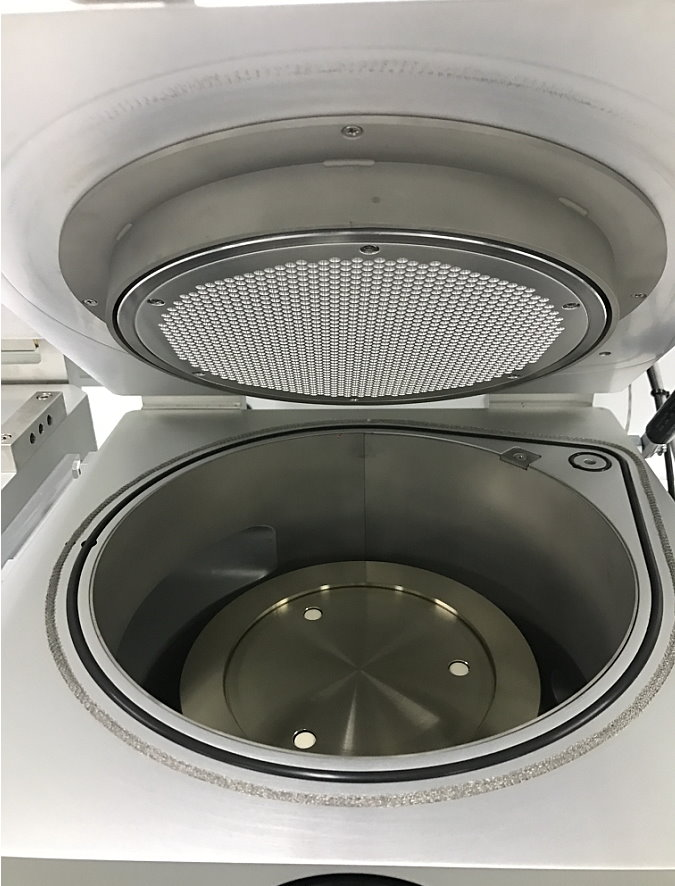
\includegraphics[width=0.64\linewidth]{fig_pecvd_chamber_photo}
\caption{Open chamber of a commercial PECVD system, showing the showerhead and substrate-support region. Photograph from Syskey Technology Co., Ltd. \citep{syskey2026pecvd}. The photograph illustrates PECVD hardware; Fig.~\ref{fig:system-en-new} defines the modeled equipment topology.}
\label{fig:pecvd-photo-en}
\end{figure}

The proposed integration interface uses material and resource identifiers to associate planned actions with resource states and completion events. These fields support subsequent controller mapping and remaining-task rescheduling. The computational study evaluates offline schedules generated from initial batch states and prescribed parameter perturbations.

Inputs comprise (1) batches, wafer identities, material sources, and modes; (2) recipe durations, residency bounds, cleaning rules, topology, capacities, and action times; (3) initial equipment positions, dummy inventory, and resource availability; and (4) total and stage budgets and termination conditions. Each output event specifies its identifier, wafer or PW, resource, origin and destination, planned start and finish, predecessor, chamber, and mode. The output also reports $C_{\max}$, waiting and cadence measures, incumbent objective value, dual bound, terminal gap, and feasibility and optimality status.

After validation against the frozen model, the schedule is exported as timed actions covering LP release and return, ATR handling, AL alignment, load-lock loading, pumping, venting and unloading, VTR handling, chamber rotation, processing, and cleaning. Each record includes its action type, resource, wafer or PW, origin and destination, planned time, and duration. Deployment requires an equipment adapter that maps these fields to tool-specific protocols and checks controller interlocks and execution timing. The exported records and validation status form the input to this adapter.

\subsection{PW-pair modeling for the two process modes}

The equipment cell is represented as a three-layer mapping from configuration
inputs through operating decisions to execution outputs. Inputs include product
wafer counts and modes, material-source interfaces, equipment action times,
cleaning intervals, residency limits, load-lock capacity, and dummy inventory.
The operating decisions jointly determine product and dummy routes, the start
and finish of every physical action, and the order of shared-resource use. The
output is a complete finite-batch timeline together with its feasibility and
optimality status. The boundary covers the product path from an LP through
processing and back to an LP and the closed dummy loop from vacuum storage
through filling or cleaning and back to storage. No buffer outside the LP,
aligner, load locks, rotating chambers, and dummy storage is assumed; every wait
therefore corresponds to an explicit physical-occupancy interval.

A wafer pair (PW pair) is a physical two-wafer transport and chamber-occupancy unit. Its members may be product+product (product PW pair), dummy+dummy (dummy PW pair), or product+dummy (mixed PW pair). Product wafers are preferentially paired by mode and index; an odd tail product may be paired with one dummy, while full-occupancy filling and cleaning may use dummy PW pairs. The sets $\mathcal P^F$ and $\mathcal P^L$ index product-containing PW pairs, including product PW pairs and any required mixed PW pairs. Alignment and residency remain wafer-level operations; the two members share a time window only on a selected two-hand transfer or the same chamber side. Preprocessing specifies product-containing PW pairing and compatible chamber positions. The MILP optimizes the remaining activation and assignment decisions, physical dummy identities, paired transfers, resource order, and event times within this layout. Legal cleaning segments are generated from the cleaning interval and complete recipe boundaries, after which the MILP activates the cleaning tasks and schedules their times.

A product follows LP--ATR--AL--ATR--upper load lock--VTR--rotary chamber--VTR--lower load lock--ATR--LP: the ATR first places the wafer on the aligner, then retrieves it for transfer into the vacuum domain. A dummy travels from vacuum storage through the VTR to the chamber and returns through the VTR after use. A regular all-product $4\times1$ batch contains two product PW pairs, hence four product wafers, and processes all four positions synchronously once before last-in--first-out unloading; only the last incomplete batch may use a dummy or mixed PW pair to fill all positions. In $2\times2$, every product-containing PW pair occupies two adjacent process cycles so that each of its product members is processed twice. For three product PW pairs, a dummy PW pair D is loaded first, the chamber rotates, and P1 is loaded before D+P1 undergoes chamber processing. Chamber processing then alternates with ``chamber rotation + chain slide'', changing the occupancy successively to P1+P2, P2+P3, and P3+D; P1, P2, and P3 are each processed twice before all wafers are unloaded. Figures~\ref{fig:chain-en} and \ref{fig:parallel-en} show the event sequences.

\begin{figure}[t]
\centering
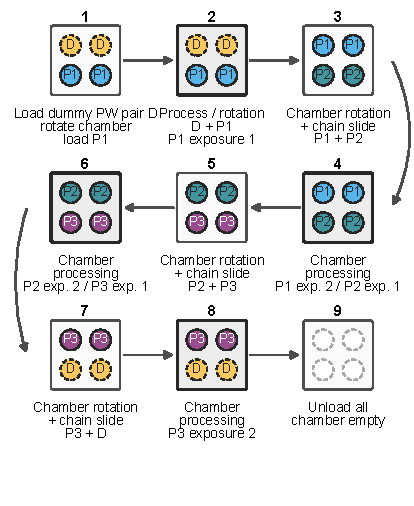
\includegraphics[width=\linewidth]{fig_chain_en_nature}
\caption{$2\times2$ chained processing. A PW pair may be P+P, D+D, or P+D; here each P$i$ is a P+P product PW pair and D is a D+D dummy PW pair. Step 1 loads D, rotates the chamber, and loads P1; Step 2 performs chamber processing on D+P1; Step 3 applies chamber rotation + chain slide to obtain P1+P2. Repeating ``chamber processing--chamber rotation + chain slide'' makes P1, P2, and P3 participate in two adjacent process cycles, so every product wafer is processed twice before all wafers are unloaded.}
\label{fig:chain-en}
\end{figure}

\begin{figure}[t]
\centering
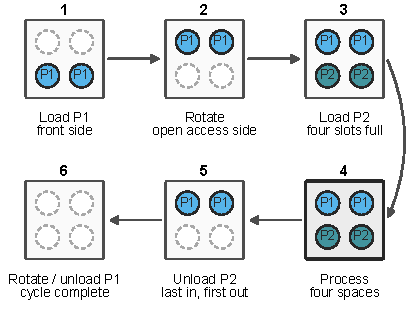
\includegraphics[width=\linewidth]{fig_parallel_en_nature}
\caption{$4\times1$ parallel processing. A regular all-product batch uses two product PW pairs, comprising four product wafers, and receives one synchronous full-occupancy process before last-in--first-out unloading; a dummy or mixed PW pair can complete the final short batch.}
\label{fig:parallel-en}
\end{figure}

Tables~\ref{tab:symbol-en-a} and \ref{tab:symbol-en-b} list every symbol in the core formulation and distinguish sets/indices, input constants, fixed binary aliases, binary decisions, continuous decisions, and derived quantities. In the implementation, $x^F$ and $x^L$ are continuous $[0,1]$ aliases fixed to zero or one by equality; this preserves uniform export names without creating extra branching decisions.

\begin{table*}[t]
\centering
\scriptsize
\setlength{\tabcolsep}{2.5pt}
\caption{Core notation I: sets, indices, and input parameters}
\label{tab:symbol-en-a}
\begin{tabular}{C{0.20\textwidth}C{0.20\textwidth}C{0.55\textwidth}}
\toprule
Symbol & Domain and role & Meaning \\
\midrule
$\mathcal S,\mathcal I$ & sets/indices & Material-source interfaces and material units; $i\in\mathcal I$ may be a product or dummy demand.\\
$\mathcal W$ & set/index & Product wafers, indexed by $w$.\\
$\mathcal P^F,\mathcal P^L$ & sets/indices & Product-containing PW pairs assigned to $4\times1$ and $2\times2$; they include P+P product pairs and any required P+D mixed pairs, indexed by $p$.\\
$\mathcal C$ & set/index & Rotary process chambers, indexed by $c$.\\
$\mathcal B_c,\mathcal K_c$ & ordered sets/indices & Candidate $4\times1$ batches $b$ and $2\times2$ product-chain positions $k$ in chamber $c$.\\
$\mathcal L=\{1,2\}$ & set/index & Front and back sides of a $4\times1$ batch.\\
$\mathcal Q_c,\mathcal E_c$ & ordered sets/indices & $2\times2$ process cycles $q$ and cleaning segments $e$ in chamber $c$.\\
$\mathcal V_c$ & set/index & Union of all $4\times1$ batches and $2\times2$ cycles in chamber $c$.\\
$\mathcal O,\mathcal A$ & sets/indices & Candidate physical operations and required process-precedence arcs.\\
$\mathcal R,\Lambda_r$ & sets/indices & Shared resources and physical slots of resource $r$.\\
$\mathcal J_c^D,\mathcal T_c$ & sets/indices & Dummy-wafer demands and reusable physical dummies of chamber $c$.\\
$\chi_{is}$ & known binary constant & Whether material unit $i$ belongs to source interface $s$.\\
$\bar x^F_{pcbl},\bar x^L_{pck}$ & known binary constants & Canonical pair-to-$4\times1$-side or pair-to-$2\times2$-position assignment.\\
$q_c^-(k),q_c^+(k)$ & known nonnegative integer maps & First and second process cycles of $2\times2$ chain position $k$, with $q_c^+(k)=q_c^-(k)+1$.\\
$\bar z_{ce},\bar a^F_{cbe},\bar a^L_{cqe}$ & known binary constants & Active cleaning segments and pre-generated membership of batches or cycles.\\
$H,\bar Q_c$ & nonnegative integer constants & Maximum cycles between cleanings and generated $2\times2$ cycles in chamber $c$.\\
$d_o,\delta_{oo'}$ & nonnegative constants & Duration of operation $o$ and minimum lag on arc $(o,o')$.\\
$d^F_\nu,d^L,r_c$ & nonnegative constants & $4\times1$ stage duration, $2\times2$ process time, and chamber half-rotation time.\\
$\rho^r_{oo'}$ & nonnegative constant & Empty travel or reset time from operation $o$ to $o'$ on resource $r$.\\
$M,\overline R_{wr}$ & positive constants & Valid horizon-based big-$M$ and maximum residency of wafer $w$ in restricted region $r$.\\
$\kappa_o,\Gamma_o$ & integer/set constants & Slots required by operation $o$ and the slots it may use.\\
$\lambda_1,\ldots,\lambda_4$ & nonnegative constants & Stage-two weights for total wait, maximum wait, cadence deviation, and soft-limit excess.\\
$\bar\omega_\alpha,\varepsilon_C$ & nonnegative constants & Soft limit for wait $\alpha$ and the stage-two makespan tolerance.\\
$\mathcal F,\mathcal D_{\rm fix}$ & sets & Full MILP feasible region and discrete indices fixed in stage two.\\
$\mathcal Q^w,\mathcal I_h$ & sets/indices & Wait quantities and process starts admitting cadence second differences.\\
\bottomrule
\end{tabular}
\end{table*}

\begin{table*}[t]
\centering
\scriptsize
\setlength{\tabcolsep}{1pt}
\caption{Core notation II: decision variables, fixed aliases, and derived quantities}
\label{tab:symbol-en-b}
\begin{tabular}{C{0.18\textwidth}C{0.15\textwidth}C{0.47\textwidth}}
\toprule
Symbol & Domain and role & Meaning \\
\midrule
$x^F_{pcbl},x^L_{pck}$ & fixed continuous $[0,1]$ aliases & Product-containing PW-pair placement on a $4\times1$ batch side or at a $2\times2$ chain position.\\
$\mu^L_{pcq}$ & fixed continuous $[0,1]$ alias & Whether $2\times2$ product-containing PW pair $p$ is processed in cycle $q$ of chamber $c$.\\
$u^F_{cb},f^F_{cbl},t^F_{cb}$ & binary variables & $4\times1$ batch activation, dummy filling on a side, and final active batch.\\
$u^L_{ck},a^L_c,v^L_{cq},h^L_{ck}$ & binary variables & $2\times2$ position, chain, process-cycle, and chain-tail activation.\\
$z_{ce},a^F_{cbe},a^L_{cqe},q^{\rm cl}_{ce}$ & fixed-binary aliases/variables & Cleaning segments, task membership, and cleaning-task activation.\\
$\tau_{ce}$ & fixed binary parameter & Whether segment $e$ is the final production segment and exactly exhausts $H$ cycles, thereby triggering terminal cleaning.\\
$q_j,g_{j\tau}$ & binary variables & Dummy demand and assignment to physical dummy $\tau$.\\
$b_o,y^r_{oo'}$ & binary variables & Operation activation and whether $o$ precedes $o'$ on resource $r$.\\
$h_{o\ell}$ & binary slot variable & Whether operation $o$ occupies physical slot $\ell$.\\
$\gamma_{pa}$ & binary variable & Whether pair $p$ uses one paired transfer on robot route $a$.\\
$s_o,e_o$ & nonnegative variables & Start and end times of operation $o$.\\
$s^{F,\nu},e^{F,\nu},s^L,e^L$ & continuous aliases & Stage-specific notation for $s_o,e_o$ in the two modes.\\
$A^F_{cb},N_{ce}$ & derived continuous/integer quantities & Product-pair count in a $4\times1$ batch and active cycles in a cleaning segment.\\
$a_{vce}$ & fixed binary alias & Whether task $v\in\mathcal V_c$ belongs to cleaning segment $e$.\\
$C_w,C_{\max}$ & nonnegative variables & Product completion time and lot makespan.\\
$\omega_\alpha,L_{\rm sum},L_{\max}$ & nonnegative variables/derived quantities & Stage-two wait or idle quantities, their sum, and their maximum.\\
$\Delta_{ceq},v_{ceq},\eta_\alpha$ & derived/nonnegative variables & Cadence second difference, its absolute-value bound, and soft wait excess.\\
$h_{ceq},\Phi$ & continuous alias/derived objective & Start of the $q$th process in a segment and stage-two schedule-quality objective.\\
$\xi,\widehat\xi,\widehat C$ & vector/stage constants & Current variables, stage-one incumbent, and incumbent makespan.\\
\bottomrule
\end{tabular}
\end{table*}

\subsection{Source interfaces, operation activation, and time relations}

The fixed incidence parameter satisfies
\begin{equation}
\sum_{s\in\mathcal S}\chi_{is}=1,
\qquad i\in\mathcal I.
\label{eq:source-membership-en}
\end{equation}
Equation~\eqref{eq:source-membership-en} assigns each material unit to exactly one source. Setting $|\mathcal S|=1$ gives the single-source tool; using two interfaces and assigning products and dummies to different interfaces gives the dual-source tool.

If $\mathcal A^{\rm int}$ is the internal network and $\mathcal A_s$ contains release and return arcs for source $s$, then
\begin{equation}
\mathcal A=\mathcal A^{\rm int}\cup
\left(\bigcup_{s\in\mathcal S}\mathcal A_s\right).
\label{eq:route-union-en}
\end{equation}
Equation~\eqref{eq:route-union-en} means that one- and two-source tools differ only at route endpoints; processing, cleaning, shared resources, and timing use the same internal model, so a dual-source tool is not the sum of two independent single-source schedules.

Canonical pair positions satisfy
\begin{equation}
\begin{aligned}
x^F_{pcbl}&=\bar x^F_{pcbl}, &
\sum_{c,b,l}x^F_{pcbl}&=1 &&(p\in\mathcal P^F),\\
x^L_{pck}&=\bar x^L_{pck}, &
\sum_{c,k}x^L_{pck}&=1 &&(p\in\mathcal P^L).
\end{aligned}
\label{eq:pair-slot-en}
\end{equation}
Equation~\eqref{eq:pair-slot-en} assigns each wafer pair to one compatible position and fixes equivalent locations to canonical indices. Event times and resource order remain optimization decisions within the prescribed layout.

A position containing a pair must be active, and candidate positions are used consecutively:
\begin{equation}
\begin{aligned}
x^F_{pcbl}&\le u^F_{cb}, &u^F_{c,b+1}&\le u^F_{cb},\\
x^L_{pck}&\le u^L_{ck}, &u^L_{c,k+1}&\le u^L_{ck}.
\end{aligned}
\label{eq:activation-prefix-en}
\end{equation}
Equation~\eqref{eq:activation-prefix-en} activates any batch or chain position containing a product and excludes a nonphysical inactive position followed by an active one.

For each candidate operation $o$, activation and duration satisfy
\begin{equation}
0\le s_o\le Mb_o,\qquad
0\le e_o\le Mb_o,\qquad
e_o=s_o+d_ob_o.
\label{eq:operation-time-en}
\end{equation}
Equation~\eqref{eq:operation-time-en} sets inactive operation times to zero and gives an active operation duration $d_o$. It applies to robot moves, alignment, pump/vent, rotation, product processing, dummy transport, and cleaning.

For every required process arc $(o,o')\in\mathcal A$,
\begin{equation}
b_{o'}\le b_o,\qquad
s_{o'}\ge e_o+\delta_{oo'}-M(2-b_o-b_{o'}).
\label{eq:precedence-en}
\end{equation}
Equation~\eqref{eq:precedence-en} activates a successor only with its predecessor and, when both exist, starts it after the predecessor and minimum lag. These arcs connect product routes, dummy routes, and load--process--unload chains.

\subsection{Occupancy and event order in the two processing modes}

For $4\times1$, let $A^F_{cb}=\sum_{p,l}x^F_{pcbl}$ be the number of product pairs assigned to batch $(c,b)$. Full occupancy and dummy filling are
\begin{equation}
\begin{aligned}
A^F_{cb}&=\sum_{p\in\mathcal P^F}\sum_{l\in\mathcal L}x^F_{pcbl},\\
\sum_{p\in\mathcal P^F}x^F_{pcbl}+f^F_{cbl}&=u^F_{cb}
&& (l\in\mathcal L),\\
\sum_{l\in\mathcal L}f^F_{cbl}&=2u^F_{cb}-A^F_{cb}.
\end{aligned}
\label{eq:full-capacity-en}
\end{equation}
Equation~\eqref{eq:full-capacity-en} gives each active $4\times1$ batch two sides, each occupied by one product pair or one dummy pair; all four chamber positions are therefore filled at process start.

Active batches are consecutive and dummy filling is restricted to the last active batch:
\begin{equation}
\begin{aligned}
A^F_{cb}&\ge u^F_{cb}, &u^F_{c,b+1}&\le u^F_{cb},\\
A^F_{cb}&\ge2u^F_{c,b+1},
&t^F_{cb}&\le u^F_{cb},\\
t^F_{cb}&\le1-u^F_{c,b+1},
&t^F_{cb}&\ge u^F_{cb}-u^F_{c,b+1}.
\end{aligned}
\label{eq:full-tail-en}
\end{equation}
Equation~\eqref{eq:full-tail-en} requires at least one product pair in an active batch and two product pairs if a later batch is active. The last three inequalities set $t^F_{cb}=1$ exactly at the active tail; the final candidate uses $t^F_{cB}=u^F_{cB}$.

Let $FL,BL,P,BU,FU$ denote front load, back load, processing, back unload, and front unload. Then
\begin{equation}
\begin{aligned}
e^{F,\nu}_{cb}&=s^{F,\nu}_{cb}+d^{F}_{\nu}u^F_{cb}
&&\bigl(\nu\in\{FL,BL,P,BU,FU\}\bigr),\\
s^{F,BL}_{cb}&\ge e^{F,FL}_{cb}+r_c-M(1-u^F_{cb}),\\
s^{F,P}_{cb}&=e^{F,BL}_{cb},\\
s^{F,BU}_{cb}&\ge e^{F,P}_{cb}-M(1-u^F_{cb}),\\
s^{F,FU}_{cb}&\ge e^{F,BU}_{cb}+r_c-M(1-u^F_{cb}).
\end{aligned}
\label{eq:full-sequence-en}
\end{equation}
Equation~\eqref{eq:full-sequence-en} loads the front side, rotates to load the back, starts synchronous processing after the back load, and then unloads the back side before rotating and unloading the front. Consecutive batches are linked by $s^{F,FL}_{c,b+1}\ge e^{F,FU}_{cb}-M(1-u^F_{c,b+1})$.

For $2\times2$, each product pair occupies one ordered chain position:
\begin{equation}
u^L_{ck}=\sum_{p\in\mathcal P^L}x^L_{pck},\qquad
u^L_{c,k+1}\le u^L_{ck},\qquad
a^L_c=u^L_{c1}.
\label{eq:mix-position-en}
\end{equation}
Equation~\eqref{eq:mix-position-en} creates a one-to-one relation between product pairs and consecutive chain positions and uses $a^L_c$ to indicate whether chamber $c$ contains a $2\times2$ chain.

Let $q_c^-(k)$ and $q_c^+(k)$ denote the first and second process cycles of chain position $k$. The pair--cycle incidence is
\begin{equation}
\begin{aligned}
q_c^+(k)&=q_c^-(k)+1,\\
\mu^L_{pcq}
&=\sum_{\substack{k\in\mathcal K_c:\\q\in\{q_c^-(k),q_c^+(k)\}}}x^L_{pck},\\
\sum_{q\in\mathcal Q_c}\mu^L_{pcq}
&=2\sum_{k\in\mathcal K_c}x^L_{pck}.
\end{aligned}
\label{eq:mix-two-exposures-en}
\end{equation}
Equation~\eqref{eq:mix-two-exposures-en} maps every assigned $2\times2$ product-containing PW pair to exactly two adjacent process cycles. Every product member inherits the same $\mu^L_{pcq}$ incidence, so a product is not omitted even when an odd tail uses a P+D mixed PW pair. The equation also distinguishes the modes explicitly: a $2\times2$ product-containing pair spans two cycles, whereas two $4\times1$ side pairs are processed once in one full batch.

The generated layout supplies the number $\bar Q_c$ of process cycles, and $h^L_{ck}$ identifies the chain tail:
\begin{equation}
\begin{aligned}
v^L_{cq}&=
\begin{cases}a^L_c,&q\le\bar Q_c,\\0,&q>\bar Q_c,
\end{cases}\\
\sum_k h^L_{ck}&=a^L_c,\qquad
h^L_{ck}\le u^L_{ck},\qquad
h^L_{ck}+u^L_{c,k+1}\le1,\\
h^L_{ck}&\ge u^L_{ck}-u^L_{c,k+1}.
\end{aligned}
\label{eq:mix-layout-en}
\end{equation}
Equation~\eqref{eq:mix-layout-en} gives $n+1$ process cycles for a segment with $n$ product-containing PW pairs: the head is dummy PW pair+P1, internal cycles are P$i$+P$i+1$, and the tail is P$n$+dummy PW pair. The final relations make $h^L_{ck}$ one only at the last active product position.

For a legal chain segment $(q_0,\ldots,q_T)$, let $H_0$, $B_q$, and $T_0$ denote head loading, internal exchange, and tail unloading. Then
\begin{equation}
\begin{aligned}
e^L_{cq}-s^L_{cq}&=d^L v^L_{cq},\\
s^L_{cq_0}&=e^{H_0}_c,\\
s^{B}_{cq}&\ge e^L_{c,q-1}-M(1-a^L_c),\qquad
s^L_{cq}=e^{B}_{cq}\quad(q_0<q\le q_T),\\
s^{T_0}_c&\ge e^L_{cq_T}-M(1-a^L_c).
\end{aligned}
\label{eq:mix-sequence-en}
\end{equation}
Equation~\eqref{eq:mix-sequence-en} begins the first process immediately after head loading, performs an internal exchange only after the previous cycle, and unloads the tail only after the last process. It directly realizes dummy+P1, P1+P2, $\ldots$, Pn+dummy.

\subsection{Cleaning and reusable dummy wafers}

Cleaning segments are generated from $H$ and complete process boundaries and enter the MILP as fixed binary aliases:
\begin{equation}
z_{ce}=\bar z_{ce},\qquad
a^F_{cbe}=\bar a^F_{cbe}u^F_{cb},\qquad
a^L_{cqe}=\bar a^L_{cqe}v^L_{cq}.
\label{eq:clean-layout-en}
\end{equation}
Equation~\eqref{eq:clean-layout-en} prevents arbitrary cleaning locations: $4\times1$ may split only at batch boundaries and $2\times2$ only after a complete chain segment, while the MILP still schedules process and cleaning times.

Let $N_{ce}$ be the number of active process cycles in segment $e$:
\begin{equation}
\begin{gathered}
N_{ce}=\sum_b a^F_{cbe}+\sum_q a^L_{cqe},\qquad
z_{ce}\le N_{ce}\le Hz_{ce},\\
q^{\rm cl}_{ce}=z_{c,e+1}+\tau_{ce},\qquad z_{c,E_c+1}=0.
\end{gathered}
\label{eq:clean-count-en}
\end{equation}
Equation~\eqref{eq:clean-count-en} places at least one and at most $H$ process cycles in an active segment. It activates an internal cleaning before every subsequent production segment and, when the final segment exactly exhausts $H$ cycles, sets $\tau_{ce}=1$ to activate terminal cleaning. Both are complete equipment actions; only the terminal action has no subsequent product processing.

Let $\mathcal V_c$ be the union of $4\times1$ batches and $2\times2$ cycles and let $a_{vce}$ take the corresponding $a^F$ or $a^L$. Cleaning order and the physical cleaning chain satisfy
\begin{equation}
\begin{aligned}
s_v&\ge e^{\rm cl}_{c,e-1}-M(1-a_{vce}) &&(e>1),\\
e_v&\le s^{\rm cl}_{ce}+M(1-a_{vce})+M(1-q^{\rm cl}_{ce}),\\
s^{\rm cl,BL}_{ce}&\ge e^{\rm cl,FL}_{ce}+r_c-M(1-q^{\rm cl}_{ce}),\\
s^{\rm cl,P}_{ce}&\ge e^{\rm cl,BL}_{ce}-M(1-q^{\rm cl}_{ce}),\\
s^{\rm cl,BU}_{ce}&\ge e^{\rm cl,P}_{ce}-M(1-q^{\rm cl}_{ce}),\\
s^{\rm cl,FU}_{ce}&\ge e^{\rm cl,BU}_{ce}+r_c-M(1-q^{\rm cl}_{ce}).
\end{aligned}
\label{eq:clean-time-en}
\end{equation}
Equation~\eqref{eq:clean-time-en} starts a segment after the preceding cleaning and finishes it before the next cleaning. A cleaning task loads both chamber sides with dummies, rotates, processes, and unloads in reverse, thereby occupying the VTR, chamber, and four physical dummies rather than adding virtual downtime.

Dummy demand $j$ is activated by a physical event:
\begin{equation}
q_j=
\begin{cases}
f^F_{cbl},&j\text{ is a final-$4\times1$ filling demand},\\
a^L_c,&j\text{ is a $2\times2$ head or tail demand},\\
q^{\rm cl}_{ch},&j\text{ is a cleaning demand}.
\end{cases}
\label{eq:dummy-demand-en}
\end{equation}
Equation~\eqref{eq:dummy-demand-en} prevents dummies from becoming an unlimited abstract filler: a physical demand exists only for a final batch, chain head/tail, or active cleaning task.

Each active demand selects one physical dummy from inventory:
\begin{equation}
\sum_{\tau\in\mathcal T_c}g_{j\tau}=q_j,
\qquad j\in\mathcal J_c^D.
\label{eq:dummy-assign-en}
\end{equation}
Equation~\eqref{eq:dummy-assign-en} assigns every active demand exactly once. Mutual exclusion subsequently orders repeated uses of the same physical dummy, so it can be reused only after unloading and return to storage.

\subsection{Robots, load locks, chambers, and time resources}

ATR, AL, VTR, and each rotary chamber are unary resources; the upper and lower load locks each have two physical slots; each dummy in inventory is a reusable slot. An operation $o$ requiring $\kappa_o$ slots satisfies
\begin{equation}
\sum_{\ell\in\Gamma_o}h_{o\ell}=\kappa_ob_o.
\label{eq:slot-select-en}
\end{equation}
Equation~\eqref{eq:slot-select-en} assigns an active operation the required number of legal physical slots and assigns none to an inactive operation. AL, ATR, VTR, and a chamber have one slot, while load locks and dummy inventory retain physical identities.

If operations $o$ and $o'$ may compete for slot $\ell$ of resource $r$, then
\begin{equation}
\begin{aligned}
s_{o'}&\ge e_o+\rho^r_{oo'}-M(1-y^r_{oo'})
-M(1-h_{o\ell})-M(1-h_{o'\ell}),\\
s_o&\ge e_{o'}+\rho^r_{o'o}-My^r_{oo'}
-M(1-h_{o\ell})-M(1-h_{o'\ell}).
\end{aligned}
\label{eq:resource-order-en}
\end{equation}
Equation~\eqref{eq:resource-order-en} makes $y^r_{oo'}$ choose one order whenever two actions use the same slot and includes empty robot travel or equipment reset through $\rho^r_{oo'}$. It applies to ATR, AL, both load locks, VTR, rotary chambers, and individual dummies, preventing concurrent robot actions and reuse before release.

An individual product or dummy stage must coincide with its selected batch, chain position, or cleaning window. For selection $x$ and reference stage $[s^{\rm ref},e^{\rm ref}]$,
\begin{equation}
\begin{aligned}
-M(1-x)&\le s_o-s^{\rm ref}\le M(1-x),\\
-M(1-x)&\le e_o-e^{\rm ref}\le M(1-x).
\end{aligned}
\label{eq:stage-link-en}
\end{equation}
Equation~\eqref{eq:stage-link-en} synchronizes the individual action with its physical stage when $x=1$ and releases the candidate relation when $x=0$, connecting pair positions, product routes, dummy demands, and chamber windows.

If pair $p$ uses one paired transfer on robot route $a$, the two wafer stages are synchronized:
\begin{equation}
\begin{aligned}
-M(1-\gamma_{pa})&\le s_{w_1a}-s_{w_2a}\le M(1-\gamma_{pa}),\\
-M(1-\gamma_{pa})&\le e_{w_1a}-e_{w_2a}\le M(1-\gamma_{pa}).
\end{aligned}
\label{eq:double-transfer-en}
\end{equation}
Equation~\eqref{eq:double-transfer-en} means that $\gamma_{pa}=1$ moves a complete pair in one non-preemptive robot action. If $\gamma_{pa}=0$, the wafers still occupy the same robot separately and are ordered by Eq.~\eqref{eq:resource-order-en}.

For the entry and exit events of wafer $w$ in restricted equipment region $r$,
\begin{equation}
0\le s_{\operatorname{out}(w,r)}-e_{\operatorname{in}(w,r)}
\le\overline R_{wr}.
\label{eq:residence-en}
\end{equation}
Equation~\eqref{eq:residence-en} limits the physical stay in an upper load lock, chamber, lower load lock, or restricted transport region. Load-lock occupation also spans placement, pump/vent, opposite-side pickup, and pressure reset, so placement by a robot is not mistaken for slot release.

\subsection{Makespan-first two-stage optimization}

Let $C_w$ be the time at which product wafer $w$ completes the lower-load-lock return and reaches its load port. Stage one solves
\begin{equation}
C_w=e_{w,\mathrm{return}},\qquad
C_{\max}\ge C_w\ (w\in\mathcal W),\qquad
\min_{\xi\in\mathcal F}C_{\max}.
\label{eq:primary-objective-en}
\end{equation}
Equation~\eqref{eq:primary-objective-en} measures makespan at the last product wafer's return to LP after its complete end-to-end route. Internal cleaning affects $C_{\max}$ through resource occupancy and precedence that delay subsequent product returns. Terminal cleaning remains in the action sequence, but its completion time does not directly lower-bound $C_{\max}$. It can still affect other chambers' product returns through competition for the shared VTR; this indirect effect is determined by the complete schedule. WPH uses product-return makespan as its denominator. The feasible region $\mathcal F$ is defined by Eqs.~\eqref{eq:source-membership-en}--\eqref{eq:residence-en} expanded over all applicable indices.

Given stage-one incumbent $\widehat\xi$ and makespan $\widehat C$, stage two fixes the discrete structure indexed by $\mathcal D_{\rm fix}$ and minimizes linear schedule quality within the makespan tolerance:
\begin{equation}
\begin{gathered}
\xi_d=\widehat\xi_d\quad(d\in\mathcal D_{\rm fix}),\qquad
C_{\max}\le\widehat C+\varepsilon_C,\\
L_{\rm sum}=\sum_{\alpha\in\mathcal Q^w}\omega_\alpha,\qquad
L_{\max}\ge\omega_\alpha,\\
\Delta_{ceq}=(h_{ce,q+1}-h_{ceq})-(h_{ceq}-h_{ce,q-1}),\\
v_{ceq}\ge\Delta_{ceq},\qquad v_{ceq}\ge-\Delta_{ceq},\\
\eta_\alpha\ge\omega_\alpha-\bar\omega_\alpha,\qquad
\eta_\alpha\ge0,\\
\min\Phi=\lambda_1L_{\rm sum}+\lambda_2L_{\max}
+\lambda_3\sum_{(c,e,q)\in\mathcal I_h}v_{ceq}
+\lambda_4\sum_{\alpha\in\mathcal Q^w}\eta_\alpha.
\end{gathered}
\label{eq:secondary-objective-en}
\end{equation}
Equation~\eqref{eq:secondary-objective-en} preserves the stage-one makespan bound and fixes the principal discrete routes and resource orders. Retained paired-transfer choices and continuous times can change to reduce total wait, maximum wait, and variation between consecutive processing intervals within each segment. Optional soft-limit excess can also be penalized. The experiments use $(\lambda_1,\lambda_2,\lambda_3)=(1,10,25)$ and $\varepsilon_C=10^{-6}$. With the soft waiting limit disabled, no excess variables are generated. For a time-limited first stage, the best incumbent value $\widehat C$ supplies the second-stage bound; variables in $\mathcal D_{\rm fix}$ are fixed while designated paired-transfer variables remain adjustable.

\subsection{Coverage and model boundary}

After index expansion, Eqs.~(1)--(25) jointly describe the finite-batch dual-source problem with mixed $4\times1/2\times2$ operation, periodic cleaning, and finite dummy inventory. Equations~(1)--(2) encode source interfaces: one interface is single source, while two interfaces with products and dummies assigned separately are dual source. Equations~(3)--(6) encode locations, activation, durations, and precedence for product-containing PW pairs. Equations~(7)--(9) encode a $4\times1$ full batch formed by two chamber-side PW pairs, final-batch filling, rotation, and last-in--first-out unloading. Equations~(10)--(13) encode the consecutive $2\times2$ chain, two adjacent exposures per product-containing PW pair, dummy-PW-pair head/tail filling, and internal exchange. Equations~(14)--(16) encode legal cleaning boundaries, segment capacity, and the physical cleaning chain. Equations~(17)--(18) encode dummy demand and finite inventory. Equations~(19)--(23) encode mutual exclusion of robots, load locks, chambers, and dummies, paired transfer, and residency. Equations~(24)--(25) encode end-to-end makespan followed by wait/cadence refinement. A pure mode is obtained by making the other mode set empty.

Every active material route has a finite precedence chain from release to return, and every pair of operations competing for one resource must be ordered. If those inequalities formed a directed cycle, summing them would require an event to occur later than itself by a positive duration, so the combination is infeasible. The resource-ordering and process-precedence constraints therefore eliminate circular waits from the schedule.

Wafer pairing, chamber-side placement, and cleaning segmentation are prescribed inputs. Optimization determines the remaining activation, assignment, transfer, ordering, and timing decisions within that layout. Mode comparisons therefore apply to the specified PW layouts and deterministic action times. Random failures and online rescheduling are outside the evaluated setting.

\section{Structure-aware MILP solution framework}
\label{sec:method-new}

The model in Section~2 must return an executable equipment timeline within a
given decision window, rather than only an objective value. On the primal side,
full occupancy, dual-source logistics, and shared-resource order can delay the
first competitive feasible plan. On the dual side, generic cut scores do not
reveal whether a cut mainly tightens discrete choices, continuous event times,
or their coupling. We first construct a feasible starting point with a
structure-preserving binary skeleton (SPBS), and then use \method{} to select
cuts in SCIP separation callbacks. SPBS improves finite-time plan availability,
and \method{} controls cut counts and insertion order, while SCIP retains responsibility for
feasibility checks, valid-cut generation, bounds, and optimality proofs
\citep{achterberg2009scip,bestuzheva2023scip}.

The complete workflow comprises six stages: construct and validate an initial solution, generate candidate cuts, predict the cut count, search for an ordered cut set, complete its structure, and resume exact search. The learning component neither generates inequalities nor changes candidate-cut coefficients; it determines only the retained prefix and input order of rows already validated by SCIP. The learned policy operates at the search-control layer; SCIP validates schedules and certifies optimality.

\subsection{SPBS initial solution}

SPBS first constructs a discrete skeleton from the recipe and equipment layout, then solves for event times in a restricted MILP. Product wafers are paired in input order. The $4\times1$ pairs are mapped sequentially to chambers, batches, and front/back positions, whereas the $2\times2$ pairs are assigned round-robin to chamber-chain positions. This determines batch-use, tail-batch, used-position, and last-position indicators. Cleaning counts partition each chamber sequence into process segments: $4\times1$ batches are assigned to their cleaning epochs, while a $2\times2$ chain ends its current segment with process-enabling carriers (PECs) when the cleaning threshold is reached and resumes after cleaning with a new PEC-bounded head. The skeleton therefore determines what is processed, in which chamber, and at which legal cleaning boundary; detailed PEC occupancy and all continuous event times remain governed by the MILP.

At the resource level, SPBS derives a conservative order from the same physical route. ATR first schedules $4\times1$ inputs and returns across chambers and stages the first $2\times2$ pair of a chamber immediately after that chamber's final full batch. It then advances chain inputs and returns segment by segment. Deterministic odd/even load-lock slots break slot symmetry, and the VTR order is aligned with ATR batch progression and cleaning actions. Let $\mathcal F_q$ be the binary variables fixed in relaxation profile $q$, with skeleton value $\widehat x_j$. The temporary model imposes
\begin{equation}
\ell_j^{(q)}=u_j^{(q)}=\widehat x_j,\qquad j\in\mathcal F_q
\label{eq:spbs-fix-en}
\end{equation}
Equation~\eqref{eq:spbs-fix-en} fixes only the binary choices regarded as reliable in the current profile. Start, completion, and waiting times, together with resource orders outside that profile, remain free.

If the strict skeleton does not yield a feasible solution within its budget, SPBS enlarges the search space through five implemented profiles. First, \texttt{spbs\_full} fixes product/batch assignment, activation, cleaning epochs, load-lock slots, ATR/AL/LL order, and VTR order. Second, \texttt{spbs\_relaxed\_vtr} releases the high-risk VTR order. Third, \texttt{spbs\_relaxed\_ll} additionally releases load-lock order. Fourth, \texttt{spbs\_fixed\_slots} releases ATR, AL, and all remaining resource orders but retains structural assignments and slots. Fifth, \texttt{spbs\_structure\_only} also releases slots, leaving only assignment, activation, and cleaning structure fixed. For instances of at least 32 wafers, the implementation begins from fixed-slot or structure-only profiles so that more time is available for feasibility search; under a tight waiting-time cap it also retains a fully unfixed \texttt{spbs\_unrestricted} attempt.

Every profile rebuilds a temporary model, sets the objective to zero, uses feasibility emphasis, aggressive heuristics, fast presolve, no separation, and stops at the first solution. Once a physical schedule is found, the program reconstructs the full model, fixes its principal discrete and continuous values, releases only secondary stability auxiliaries, completes them, and invokes the complete SCIP solution check. Only a checked high-precision solution file is passed to the production model as an incumbent. No SPBS bound is transferred, so the production solve remains free to improve the schedule and complete the global proof. In the formal benchmark SPBS is precomputed offline; its metadata records the accepted profile and all attempts, and a SHA-256 hash of the serialized LP prevents a start from being reused on a different model. Its construction cost is excluded from reported PDI and main-solve time.

\subsection{HEM baseline and role-aware representation}

Prior learning-based cut selectors address generic candidate sets with reinforcement learning, learned ranking, and look-ahead imitation \citep{tang2020cut,huang2022cutranking,paulus2022looking}. HEM further identifies three coupled decisions---which cuts, how many cuts, and in what order---and handles them with a high-level count policy and a low-level sequence policy \citep{wang2023hem}. We retain HEM's hierarchical decomposition and pointer decoding and use its 13D implementation as the direct baseline. Training instances, budgets, random seeds, candidate limits, and hidden dimensions are shared while representation, decoding, and post-selection completion are compared. HEM was subsequently extended to hierarchical sequence/set models \citep{wang2024hemset}; HEM-13D here is a controlled reproduction of the 2023 sequence implementation.

The 13D HEM candidate vector comprises objective parallelism, efficacy, normalized support, integral-support ratio, normalized violation, the mean/maximum/minimum/standard deviation of row coefficients, and the corresponding four objective-coefficient statistics. These features describe immediate LP quality and numerical scale. They do not distinguish two similarly efficacious rows when one acts on discrete route choices and the other on continuous event times. In the present model, that distinction corresponds directly to changing a process/resource combination versus tightening the timing of an existing combination.

Starting from the 13 generic HEM features, variables are partitioned by solver metadata into binary, general integer, objective-active continuous, continuous auxiliary, and other roles. The coefficient mass of role $g$ in cut $i$ is
\begin{equation}
p_{ig}=\frac{\sum_{j:x_j\in g}|a_{ij}|}{\sum_j|a_{ij}|+\varepsilon}.
\label{eq:role-mass-en}
\end{equation}
Equation~\eqref{eq:role-mass-en} is the fraction of absolute cut-coefficient mass carried by a mathematical variable role. Beyond the five role masses, the added features are mass on variables with two finite global bounds, positive-coefficient mass, discrete--continuous coupling $4(p_{iB}+p_{iI})(p_{iC_{\rm obj}}+p_{iC_{\rm aux}})$, the largest non-residual role mass, and normalized role entropy. The resulting vector has 23 dimensions. Roles are identified solely from SCIP variable types, objective coefficients, and global bounds; neither variable names nor equipment labels are read, so variable renaming leaves the representation unchanged.

HEM uses a hierarchical ``count policy + ordered-subset policy'' decomposition: its high level predicts the number of cuts from a sequence representation, while its low level uses an LSTM encoder--decoder with pointer attention to select cuts sequentially \citep{wang2023hem,vinyals2015pointer}. Building on this hierarchy, the proposed selector introduces a role-aware grouped gated encoder before the LSTM, a role-submodular completion step after the pointer sequence, and width-three beam search during formal inference, which together form the complete RDMCT-HBS selection pipeline.


\subsection{Role-aware encoding and hierarchical sequence decoding}

Let $m_t$ be the number of candidates retained at separation callback $t$. For candidate cut $i$, write the 23D input as $x_i=[x_i^{H};x_i^{R}]$, where $x_i^{H}\in\mathbb R^{13}$ contains the generic HEM features and $x_i^{R}\in\mathbb R^{10}$ contains the proposed role-aware features. The full vector is first layer-normalized; the two feature groups are then projected separately into the common hidden space and fused by an elementwise gate generated from all 23 features:
\begin{equation}
\begin{aligned}
\widetilde x_i&=\operatorname{LN}(x_i),\\
u_i^{H}&=W_H\widetilde x_i^{H}+b_H,\qquad
u_i^{R}=W_R\widetilde x_i^{R}+b_R,\\
g_i&=\sigma(W_g\widetilde x_i+b_g),\qquad
z_i=g_i\odot u_i^{H}+(1-g_i)\odot u_i^{R}.
\end{aligned}
\label{eq:gated-encoding-en}
\end{equation}
Here $z_i\in\mathbb R^{128}$ is the fused candidate embedding. Unlike a single projection of the 23D vector, the two branches preserve generic LP quality and mathematical-role structure separately, while $g_i$ determines their candidate-specific contribution in each hidden dimension. Thus two cuts with similar efficacy but different concentration on discrete route variables or continuous timing variables can remain distinguishable. This grouped gated adapter is a structural change to HEM's input representation introduced in this work.

The fused candidates, in the deterministic order established by Step~1, are passed through a single-layer LSTM encoder:
\begin{equation}
(h_i,c_i)=\operatorname{LSTM}(z_i,h_{i-1},c_{i-1}),\qquad i=1,\ldots,m_t .
\label{eq:lstm-encoding-en}
\end{equation}
The states $h_i$ turn local cut descriptors into context-dependent candidate representations and are used by both the high-level retained-count policy and the low-level ordered selector. A 128D hidden state is used to encode the ordered candidates into a contextual sequence representation. Fixing the input order also makes the encoded sequence reproducible for an identical candidate pool.

At low-level decoding step $r$, the decoder state $d_r$ and all encoder states $h_i$ are used for one glimpse attention followed by pointer attention. Let $M_{ri}=-\infty$ if candidate $i$ already appears in the prefix and $M_{ri}=0$ otherwise. Then
\begin{equation}
\begin{aligned}
a_{ri}&=v_g^\top\tanh(W_e h_i+W_d d_r)+M_{ri},\\
\alpha_{ri}&=\operatorname{softmax}_i(a_{ri}),\\
\bar h_r&=\sum_i\alpha_{ri}h_i,\\
b_{ri}&=v_p^\top\tanh(U_e h_i+U_g\bar h_r)+M_{ri},\\
P(i_r=i\mid i_{1:r-1},S_t)&=\operatorname{softmax}_i(b_{ri}).
\end{aligned}
\label{eq:pointer-decoding-en}
\end{equation}
Equation~\eqref{eq:pointer-decoding-en} makes the sequential dependence explicit. The selected prefix updates the decoder state and the next conditional distribution. Masking excludes previously selected cuts, and the glimpse summarizes the candidate pool for the current prefix. The resulting sequence model combines contextual candidate encoding, prefix-aware pointer decoding, and the proposed representation and completion stages into one role-aware selector.

Training keeps stochastic sampling from the policy for exploration. During formal inference, instead of committing to one path at every step, the method maintains $B=3$ partial sequences. For parent beam $b=(i_1,\ldots,i_{r-1})$ and an unselected extension $j$, the accumulated score is
\begin{equation}
L_r(b\oplus j)=L_{r-1}(b)+\log P(i_r=j\mid b,S_t),
\label{eq:beam-score-en}
\end{equation}
All parent-beam--candidate extensions are compared and the three largest $L_r$ values are retained. After the high-level target length $k_t$ is reached, the best sequence is passed to the completion stage. This beam procedure preserves multiple high-probability partial sequences during decoding, reduces early commitment, and works jointly with the subsequent policy-anchored role-submodular completion to inject variable-role structure into the final selected set.

\subsection{Stepwise selection from candidate pool to ordered cuts}

At separation callback $t$, the method executes the following sequence.

\noindent\textbf{Step 1: form the candidate pool.} SCIP first generates and validates candidate rows $\mathcal C_t$ with its own separators. To avoid traversing the complete sparse support of thousands of rows, the method uses SCIP's inexpensive efficacy accessor to retain at most 128 candidates. Ties are broken by original index for deterministic input. Forced cuts remain under solver control and are not placed in the learned ranking.

\noindent\textbf{Step 2: compute and encode the state.} The 13 HEM and 10 role-aware features are extracted for every row, with role masses, dominant role, and structural entropy retained as metadata. Equation~\eqref{eq:gated-encoding-en} then performs grouped gated fusion and Eq.~\eqref{eq:lstm-encoding-en} produces contextual candidate states. The encoded candidate set is $S_t$.

\noindent\textbf{Step 3: determine the retained count.} The high-level policy outputs a tanh-bounded action in $[-1,1]$, which is mapped to a retained fraction $\rho_t$. The fraction is then clipped by the global 0.2 cap, SCIP's round-specific limit, and the implementation cap of 16 cuts, producing $k_t$. When enough candidates exist, at least two rows are retained to prevent repeated callbacks from degenerating to an empty selection.

\noindent\textbf{Step 4: construct the candidate order.} At low-level step $r$, the pointer policy conditions on $S_t$ and the selected prefix $i_{1:r-1}$ to score all remaining candidates. Selected indices are masked with negative infinity and cannot be repeated. The joint high- and low-level policy is
\begin{equation}
\pi_\theta(k_t,i_{1:k_t}\mid S_t)=\pi_\theta^H(k_t\mid S_t)
\prod_{r=1}^{k_t}\pi_\theta^L(i_r\mid S_t,i_{1:r-1}).
\label{eq:policy-en}
\end{equation}
Equation~\eqref{eq:policy-en} means that the high level determines the sequence length and the low level then chooses distinct candidates within that length. Each earlier cut changes both the remaining action set and the decoder state used by later probabilities.

\noindent\textbf{Step 5: beam decoding.} The low-level policy samples stochastically during training. At test time, beam search of width three is used. At step $r$, every partial sequence is extended by every unselected candidate; joint log-probabilities are accumulated, and the three highest-scoring items over all parent-beam--next-candidate pairs are retained. After $k_t$ steps, the best sequence is returned. Unlike one-step greedy decoding, the beam retains an initially lower-ranked prefix whose later joint probability can be higher. This fixed-width neural construction follows the broader use of beam decoding in neural combinatorial optimization \citep{choo2022beam}.

\noindent\textbf{Step 6: role-submodular completion.} A sequence based only on joint probability can still repeatedly cover one variable role. The first $\lceil0.25k_t\rceil$ pointer candidates are retained as policy anchors. The remaining policy order is merged with a heuristic tail sorted by instantaneous structural quality $q_i$, and at most $2k_t$ rows form expansion pool $\mathcal R_t$. For $S\subseteq\mathcal R_t$, define
\begin{equation}
\begin{aligned}
F_t(S)={}&\sum_{i\in S}(0.35q_i+0.20r_i)
+0.25\sum_{g\in\mathcal G}d_g\sqrt{\sum_{i\in S}p_{ig}}\\
&+\frac{0.20}{|\mathcal R_t|}\sum_{u\in\mathcal R_t}\max_{i\in S}s_{ui},
\end{aligned}
\label{eq:submodular-en}
\end{equation}
where $r_i$ is the normalized pointer-rank prior, $d_g$ is the demand share of role $g$ in the expansion pool, and $s_{ui}$ is clipped cosine similarity on generic-quality and role-mass descriptors. The score $q_i$ combines efficacy, violation, integral support, recognized-role ratio, dominant-role ratio, and structural entropy. In Eq.~\eqref{eq:submodular-en}, the first term retains instantaneous quality and the learned order; the square-root coverage term gives diminishing marginal gain to repeated role mass; and the final term makes the selected cuts represent the main structures in the pool. Starting from the anchors, the method recomputes the marginal gain of every unselected candidate and adds the largest until $k_t$ cuts have been selected. The nonnegative modular, concave-over-modular, and facility-location terms form a monotone submodular objective, so the residual greedy completion after fixing anchors and the expansion pool inherits the standard $1-1/e$ approximation property \citep{nemhauser1978analysis}.

Finally, the $k_t$ selected rows are placed at the front of the returned array in the chosen order, while all other candidates remain as an unselected suffix. SCIP adds only the prefix to the current LP. One callback therefore completes six operations: inexpensive truncation, feature extraction, count prediction, sequence decoding, structural completion, and return to SCIP.

\begin{table}[!htbp]
\raggedright
\scriptsize
\setlength{\tabcolsep}{3pt}
\algorithmtitle{Cut selection by parallel hierarchical REINFORCE and beam search}
\label{alg:cut-selection-en}
\begin{tabular}{>{\raggedright\arraybackslash}p{0.92\columnwidth}}
\toprule
\textbf{Algorithm steps}\\
\midrule
\textbf{Input:} SCIP-validated rows $\mathcal C_t$, high-level policy $\pi_\theta^H$, low-level pointer policy $\pi_\theta^L$, beam width $B=3$, and the current SCIP cut limit.\\
\textbf{Output:} Ordered cut prefix $S_t^\star=(i_1,\ldots,i_{k_t})$ and the unselected suffix returned to SCIP.\\
\textbf{1. Train the policies.} Two workers collect rollouts in parallel with terminal reward $R=-\pdi$; a central learner applies hierarchical REINFORCE with separate EMA baselines and synchronous Adam updates. Fix the parameters for formal inference.\\
\textbf{2. Form the pool.} Sort by efficacy, break ties by original index, and retain at most 128 rows.\\
\textbf{3. Encode the state.} Compute 13 HEM features, ten role-aware features, and role-mass metadata; apply grouped projections, sigmoid-gated fusion, and LSTM encoding.\\
\textbf{4. Determine the count.} Predict the retained fraction with $\pi_\theta^H$ and obtain $k_t$ after the 0.2 fraction cap, SCIP round limit, and 16-cut implementation cap.\\
\textbf{5. Initialize the beam.} Set $\mathcal B_0$ to the empty sequence with log probability zero.\\
\textbf{6. Expand.} For $r=1,\ldots,k_t$, obtain masked conditional probabilities from one glimpse plus pointer attention, extend every prefix in $\mathcal B_{r-1}$ by every unselected candidate, and accumulate log probability.\\
\textbf{7. Prune.} Retain the three highest joint-probability parent--candidate extensions as $\mathcal B_r$; after the loop, take the leading sequence in $\mathcal B_{k_t}$.\\
\textbf{8. Fix anchors.} Retain its first $\lceil0.25k_t\rceil$ rows as policy anchors $A_t$.\\
\textbf{9. Form the expansion pool.} Merge the remaining pointer order with structural-quality order, remove duplicates, and keep at most $2k_t$ rows as $\mathcal R_t$.\\
\textbf{10. Complete submodularly.} Set $S\leftarrow A_t$; while $|S|<k_t$, add the $i\in\mathcal R_t\setminus S$ maximizing $F_t(S\cup\{i\})-F_t(S)$.\\
\textbf{11. Return.} Return $S_t^\star$ in anchor-then-completion order; leave all other rows in the suffix and outside the current LP.\\
\bottomrule
\end{tabular}
\end{table}

\subsection{Reinforcement-learning training and exact-solver interface}

One time-limited SCIP solve forms a rollout, with its terminal PDI used as the cost. The current policy is executed in every eligible cut-selection callback. For replay, the agent records the high-level fraction and low-level sampled sequence at the first valid candidate set of that rollout, and the PDI of the complete solve is returned to both policies. Writing $R=-\pdi$ as a reward, the low-level estimator is
\begin{equation}
\begin{aligned}
\widehat{\nabla_\theta J}
&=\frac1B\sum_{b=1}^B(R_b-\bar R_{\rm EMA})
\nabla_\theta\log\pi_\theta(\tau_b),\\
\bar R_{\rm EMA}&\leftarrow0.9\bar R_{\rm EMA}+0.1\bar R.
\end{aligned}
\label{eq:reinforce-en}
\end{equation}
Equation~\eqref{eq:reinforce-en} gives the batch policy-gradient update formed from the first eligible candidate-set action record and an exponential-moving-average baseline; $B$ is the rollout batch and $\tau_b$ is the recorded cut sequence in rollout $b$. Equivalently, the code minimizes PDI-cost advantage times log probability. Low-level log probability is averaged over sequence length so that a longer cut sequence does not produce a larger gradient merely because it contains more terms. The high-level policy uses the same PDI cost and an independent EMA baseline and is updated every two epochs; both gradient norms are clipped at 2. Parallel environments collect rollouts, and a central learner updates both policies synchronously after each batch, forming a parallel hierarchical REINFORCE procedure \citep{williams1992reinforce,mnih2016a3c}.

Training uses five instances and five random seeds. Each seed has two workers, each completing four 30-s/1024-MB rollouts per epoch, for eight rollouts per epoch and 60 epochs. Initial Adam learning rates are $10^{-4}$ for the low-level policy and $5\times10^{-4}$ for the high-level policy and are multiplied by 0.96 every ten epochs. Training uses stochastic decoding and formal inference uses beam width three. Every configuration--seed combination uses the fixed epoch-60 parameters without benchmark- or test-set checkpoint selection. HEM-13D, feature-only 23D, and the complete 23D method are trained separately so that weights are never mixed across input semantics or completion environments.

\method{} only orders and selects valid rows already generated by SCIP, and SPBS submits only solutions checked in the complete model. Neither changes the objective, constraints, integrality, or bound logic. The learned components therefore change the search path and finite-time bound convergence, whereas feasibility and optimality retain the same meaning as in default SCIP.

\section{Manufacturing-system experiments and decision analysis}
\label{sec:results-new}

\subsection{Experimental design and metrics}

The experiments follow the manufacturing-system decision chain and address four
questions. First, can configuration inputs be mapped consistently to a complete
timeline satisfying dual-source routes, full occupancy, cleaning, and
shared-resource constraints while identifying the preferred mode under equal
total processing time and different cleaning frequencies? Second, after the throughput structure is determined, does two-stage
optimization improve waiting and cadence under the same total budget? Third, do
SPBS and structure-aware cut selection improve finite-time plan delivery and
primal--dual convergence relative to the direct HEM baseline, respectively? Fourth, can the decision chain continue
to return verifiable plans as scale, mixed-flow composition, operating
parameters, and the data distribution change? The core evidence comprises
cleaning-frequency mode checks, the direct HEM comparison, 960 paired SPBS runs,
1500 equal-budget workflow runs, 300 factorial runs, 80 one-factor sensitivity
runs, and 729 distribution-shift runs on 40--64-wafer batches. The main text
retains four resource-level Gantt charts for the same 16-wafer batch, grouped
by $H=10$ and $H=3$; each group shows both pure $4\times1$ and pure $2\times2$. They verify process overlap,
cleaning, and end-to-end completion time directly. Every incumbent used for a
reported conclusion passes both SCIP validation and an independent post-solve
check against the same serialized MILP.

OpenAI Codex assisted with research-code debugging and visualization scripts. Numerical results are produced by the recorded solver runs; event plots are generated programmatically from the validated schedules. The MILP, SCIP version, instances, and random seeds are frozen, and each comparison family uses common time and memory limits. Let $P(t)$ denote the primal bound of the minimization problem at time $t$, namely the objective value of the best incumbent, and let $D(t)$ denote the dual bound, namely the global lower bound certified by the search tree. Define $\Delta(t)=|P(t)-D(t)|$, $m(t)=\min\{|P(t)|,|D(t)|\}$, and $M(t)=\max\{|P(t)|,|D(t)|\}$. When the two bounds are finite, have the same sign, and differ, the terminal relative primal--dual gap is taken directly from SCIP \texttt{getGap()} as
\begin{equation}
G_{\rm end}=100\,\frac{\Delta(T)}{m(T)}.
\label{eq:terminal-gap-en}
\end{equation}
SCIP sets $G_{\rm end}=0$ when the bounds coincide and returns $+\infty$ when they have opposite signs or valid bounds are not both available. Equation~\eqref{eq:terminal-gap-en} normalizes by the smaller absolute bound and consequently does not cap $G_{\rm end}$ at 100\%. A value above 100\% indicates that the incumbent and the certified lower bound remain widely separated at the time limit.

SCIP uses a different bounded normalization for the primal--dual integral. Define the instantaneous integral gap as
\begin{equation}
g_{\rm PDI}(t)=100\,\frac{\Delta(t)}{M(t)},\qquad
\pdi=\int_0^T g_{\rm PDI}(t)\,\mathrm dt.
\label{eq:pdi-gap-en}
\end{equation}
Equation~\eqref{eq:pdi-gap-en} applies when the bounds are finite, have the same sign, and differ; SCIP sets $g_{\rm PDI}(t)=0$ for coincident bounds and $g_{\rm PDI}(t)=100$ otherwise. The instantaneous integral gap is therefore bounded to $[0,100]$; lower PDI means that the bound gap closes earlier. PDI is zero only if the gap is zero for almost the entire timed horizon, whereas $G_{\rm end}=0$ only states that optimality is proved at termination. Both quantities are exported directly from SCIP statistics \citep{achterberg2009scip,bestuzheva2023scip}.

The manufacturing instance is the inferential unit: random repeats are first aggregated within an instance, after which paired instance differences use nonparametric 95\% bootstrap intervals, Wilcoxon signed-rank tests, and Holm correction within each prespecified analysis family. Time-limited runs remain in the summaries so that random seeds are not treated as independent manufacturing evidence. Solver environments, budgets, tolerances, instance lists, and model parameters are recorded separately for each comparison family; random repeats are aggregated by manufacturing instance.

The numerical values in Table~\ref{tab:gantt-config-en} define the computational configuration. The product-return comparison uses equal cumulative nominal processing time: 180~s for one $4\times1$ exposure and 90+90~s for two $2\times2$ exposures. Recipe qualification is a prescribed input condition for this scheduling comparison.

Table~\ref{tab:gantt-config-en} lists the frozen configuration used to produce the representative 16-wafer Gantt charts. Two rotating chambers share the VTR, while product and dummy wafers compete for robots, load locks, and chamber spaces along their respective routes; cleaning counts, rotation, and transfer times are represented in the same MILP. Each displayed solution passes SCIP \texttt{checkSol} and an independent post-solve check before export, so the charts provide both a structural comparison and auditable feasibility evidence.

\begin{table*}[!htbp]
\centering
\scriptsize
\setlength{\tabcolsep}{2pt}
\caption{Frozen configuration for the cleaning-frequency mode experiment and representative Gantt charts under equal total nominal processing time.}
\label{tab:gantt-config-en}
\begin{tabular}{C{0.10\textwidth} C{0.29\textwidth} C{0.10\textwidth} C{0.29\textwidth}}
\toprule
Group & Parameter and value & Group & Parameter and value\\
\midrule
Rotating chambers & CH2 and CH3; two shared rotating PMs with four spaces each & Process time & 180~s for $4\times1$; 90+90~s for $2\times2$\\
Cleaning & At most $H=3$--10 effective process cycles between adjacent cleanings; pure-dummy cleaning 500~s & Chamber motion & 180$^\circ$ rotation 2~s; inter-action gap 1~s\\
ATR & One dual-hand robot, capacity 2; load/unload 4~s, complete loaded transfer 11~s & VTR & One four-hand robot, capacity 4; loaded transfer 4~s, empty reposition 4~s\\
ATR details & LL--LP empty return 6~s; PW-pair exchange at AL 8~s & AL & Capacity 1; minimum alignment occupancy 20~s per wafer\\
Load locks & LLupper pump/reset 30~s per slot; LLlower vent/reset 25~s & LL capacity & Two independent slots in each of upper and lower LLs\\
Material source & LP1--LP4, capacity 25 wafers each & Dummy wafers & Eight reusable wafers, four per chamber; storage capacity 10\\
Batch and model & Product batch size 4; 13 modeled process steps & Chamber bound & At most 15 $4\times1$ batch slots per PM\\
Model bounds & Big-$M=10000$; module and robot residency bounds 10000~s & Waiting option & Avoidable-wait hard cap 0, meaning that this optional cap is disabled\\
Objective & \texttt{compact\_resource\_idle}; process mode \texttt{auto} & Policy & Frozen training seed 1, epoch 60, 23 features\\
Decoder and cuts & Beam width 3; cut pool 128, at most 16 cuts selected per round & Solver & SCIP seed 1; Available, validated initial schedules\\
Solve and selection & Product-return objective; optimum certification and representative-schedule waiting refinement recorded separately & Export check & SCIP \texttt{checkSol} and independent validation for every solution\\
\bottomrule
\end{tabular}
\end{table*}

\subsection{Process-mode selection driven by cleaning position and lot size}

Steady-state analyses of multi-space CTs usually measure cycle time or throughput \citep{gu2024multifinger}. For finite batches, we define $C_{\max}$ as the time when the last product wafer returns to an LP and report equivalent batch output as $\mathrm{WPH}=3600|\mathcal W|/C_{\max}$. Pure $4\times1$ uses 180~s per wafer, pure $2\times2$ uses 90+90~s, and a 1:1 mixture assigns each product its mode-specific recipe. The cleaning interval $H$ counts full-occupancy cycles per chamber: a $4\times1$ batch counts once and each $2\times2$ exposure counts separately. Processing segments follow cycle limits and complete-chain boundaries, including 500-s cleaning and associated dummy loading, unloading, rotation, and transport.

Table~\ref{tab:mode-extended-en} compares cleaning endpoints; Table~\ref{tab:clean-crossover-en} gives the full $H=3$--10 grid. The $H=4$--9 experiment contains 36 configurations with training and solver seeds fixed at 1, a 14400-s main-solve limit, and stage~2 disabled. All 36 schedules pass independent validation; 35 are proven optimal. For 16 wafers at $H=5$, pure $2\times2$ reaches a feasible 907~s within that budget. A separate 28800-s solve of the same frozen instance, initialized from this schedule, improves the upper bound to 898~s, with lower bound 694~s and terminal gap 29.39\%. The improved schedule passes main-model and 4-s exchange checks. This certification updates the schedule bound and is excluded from the fixed-budget algorithm statistics. With cleaning inactive, the 16-wafer pure $2\times2$ models at $H=6$--10 are identical and have optimum 898~s.

\begin{table*}[!htbp]
\centering
\scriptsize
\setlength{\tabcolsep}{4pt}
\caption{Cleaning-endpoint comparison under equal cumulative nominal processing time. Cleaning counts sum internal and terminal cleans across both chambers. $\dagger$ marks a validated feasible makespan without an optimality proof; the corresponding WPH uses that makespan.}
\label{tab:mode-extended-en}
\begin{tabular}{cccccc}
\toprule
Lot (wafers) & $H$ & Mode & Total cleans & $C_{\max}$ (s) & WPH (wafers/h)\\
\midrule
8 & 10 & Pure $4\times1$ & 0 & 610 & 47.21\\
8 & 10 & Pure $2\times2$ & 0 & \textbf{578} & \textbf{49.83}\\
8 & 10 & 4:4 mixed & 0 & 654 & 44.04\\
8 & 3 & Pure $4\times1$ & 0 & 610 & 47.21\\
8 & 3 & Pure $2\times2$ & 2 & \textbf{578} & \textbf{49.83}\\
8 & 3 & 4:4 mixed & 1 & 654 & 44.04\\
\midrule
16 & 10 & Pure $4\times1$ & 0 & 944 & 61.02\\
16 & 10 & Pure $2\times2$ & 0 & \textbf{898} & \textbf{64.14}\\
16 & 10 & 8:8 mixed & 0 & 939 & 61.34\\
16 & 3 & Pure $4\times1$ & 0 & \textbf{944} & \textbf{61.02}\\
16 & 3 & Pure $2\times2$ & 4 & 1402 & 41.08\\
16 & 3 & 8:8 mixed & 2 & 1530 & 37.65\\
\midrule
24 & 10 & Pure $4\times1$ & 0 & 1268 & 68.14\\
24 & 10 & Pure $2\times2$ & 0 & $\mathbf{1237}^{\dagger}$ & \textbf{69.85}\\
24 & 10 & 12:12 mixed & 0 & 1250 & 69.12\\
24 & 3 & Pure $4\times1$ & 2 & \textbf{1268} & \textbf{68.14}\\
24 & 3 & Pure $2\times2$ & 6 & $2220^{\dagger}$ & 38.92\\
24 & 3 & 12:12 mixed & 4 & $2324^{\dagger}$ & 37.18\\
\bottomrule
\end{tabular}
\end{table*}
\begin{table*}[tp]
\centering
\scriptsize
\setlength{\tabcolsep}{3pt}
\caption{Makespans, cleaning counts, and preferred modes under the prescribed PW layouts for 8-, 16-, and 24-wafer lots at $H=3$--10. Times are in seconds.}
\label{tab:clean-crossover-en}
\begin{tabular}{cccccccccc}
\toprule
\multirow{2}{*}{Lot (wafers)} & \multirow{2}{*}{$H$} & \multicolumn{3}{c}{$C_{\max}$ (s)} & \multirow{2}{*}{$\Delta C_{\max}$ (s)} & \multicolumn{3}{c}{Total cleans} & \multirow{2}{*}{Preferred mode}\\
\cmidrule(lr){3-5}\cmidrule(lr){7-9}
 & & Pure $4\times1$ & Pure $2\times2$ & 1:1 mixed & & Pure $4\times1$ & Pure $2\times2$ & 1:1 mixed & \\
\midrule
8 & 3 & 610 & 578 & 654 & -32 & 0 & 2 & 1 & Pure $2\times2$\\
8 & 4 & 610 & 578 & 654 & -32 & 0 & 0 & 0 & Pure $2\times2$\\
8 & 5 & 610 & 578 & 654 & -32 & 0 & 0 & 0 & Pure $2\times2$\\
8 & 6 & 610 & 578 & 654 & -32 & 0 & 0 & 0 & Pure $2\times2$\\
8 & 7 & 610 & 578 & 654 & -32 & 0 & 0 & 0 & Pure $2\times2$\\
8 & 8 & 610 & 578 & 654 & -32 & 0 & 0 & 0 & Pure $2\times2$\\
8 & 9 & 610 & 578 & 654 & -32 & 0 & 0 & 0 & Pure $2\times2$\\
8 & 10 & 610 & 578 & 654 & -32 & 0 & 0 & 0 & Pure $2\times2$\\
\midrule
16 & 3 & 944 & 1402 & 1530 & 458 & 0 & 4 & 2 & Pure $4\times1$\\
16 & 4 & 944 & 1470 & 939 & 526 & 0 & 2 & 2 & 1:1 mixed\\
16 & 5 & 944 & 898$^{\dagger}$ & 939 & -46 & 0 & 2 & 0 & Pure $2\times2$\\
16 & 6 & 944 & 898 & 939 & -46 & 0 & 0 & 0 & Pure $2\times2$\\
16 & 7 & 944 & 898 & 939 & -46 & 0 & 0 & 0 & Pure $2\times2$\\
16 & 8 & 944 & 898 & 939 & -46 & 0 & 0 & 0 & Pure $2\times2$\\
16 & 9 & 944 & 898 & 939 & -46 & 0 & 0 & 0 & Pure $2\times2$\\
16 & 10 & 944 & 898 & 939 & -46 & 0 & 0 & 0 & Pure $2\times2$\\
\midrule
24 & 3 & 1268 & 2220$^{\dagger}$ & 2324$^{\dagger}$ & 952 & 2 & 6 & 4 & Pure $4\times1$\\
24 & 4 & 1268 & 2928$^{\dagger}$ & 1827$^{\dagger}$ & 1660 & 0 & 4 & 2 & Pure $4\times1$\\
24 & 5 & 1268 & 1769$^{\dagger}$ & 1796 & 501 & 0 & 2 & 2 & Pure $4\times1$\\
24 & 6 & 1268 & 1880$^{\dagger}$ & 1263$^{\dagger}$ & 612 & 0 & 2 & 1 & 1:1 mixed\\
24 & 7 & 1268 & 1237$^{\dagger}$ & 1250 & -31 & 0 & 2 & 0 & Pure $2\times2$\\
24 & 8 & 1268 & 1237$^{\dagger}$ & 1250 & -31 & 0 & 0 & 0 & Pure $2\times2$\\
24 & 9 & 1268 & 1237$^{\dagger}$ & 1250 & -31 & 0 & 0 & 0 & Pure $2\times2$\\
24 & 10 & 1268 & 1237$^{\dagger}$ & 1250 & -31 & 0 & 0 & 0 & Pure $2\times2$\\
\bottomrule
\end{tabular}
\par\smallskip
\parbox{0.97\textwidth}{\footnotesize Cleaning counts sum internal and terminal cleans across both chambers. $\dagger$ denotes a feasible upper bound; other times are proven optima. $\Delta C_{\max}$ subtracts the listed pure $4\times1$ time from the pure $2\times2$ time. A preferred mode is established by comparing optima or separating its feasible upper bound from competing lower bounds. The 24-wafer $H=7$ pure $2\times2$ entry uses a transferred and revalidated 1237-s schedule. Mixed-mode entries at $H=7$--10 share the 1250-s optimality certificate obtained within a 28800-s budget; their model hashes are identical. The 16-wafer $H=5$ and 24-wafer $H=3$ pure $2\times2$ entries also use 28800-s certification runs; other 24-wafer results use 7200-s experiments. Mixed-mode $H=3,5$ times use high-precision timing reoptimization of the same discrete schedule. All configurations allow pre-exchange waiting and split exchanges.}
\end{table*}

For 8 wafers, the three makespans remain 610, 578, and 654~s throughout $H=3$--10. Pure $2\times2$ is 5.25\% shorter than pure $4\times1$. At $H=3$, pure $2\times2$ and mixed operation generate two and one terminal cleans, respectively; no cleaning occurs at $H\ge4$. No internal cleaning is required at this lot size, and the ranking remains unchanged across the tested intervals.

For 16 wafers, the preferred mode changes with the interval. At $H=3$, pure $2\times2$ and mixed operation each contain two internal cleans, and pure $4\times1$ is preferred at 944~s. At $H=4$, pure $2\times2$ still requires two internal cleans, while mixed operation has only two terminal cleans and improves on pure $4\times1$ at 939~s. At $H=5$, pure $2\times2$ has only two terminal cleans and its feasible 898-s schedule is shorter than the proven optima of both competitors. Thus the preference between the pure modes switches from $4\times1$ at $H=4$ to $2\times2$ at $H=5$. At $H=6$--10, all modes avoid cleaning; the pure $2\times2$ optimum of 898~s is 4.87\% and 4.37\% shorter than pure $4\times1$ and mixed operation, respectively.

Complete-chain segmentation and cleaning position jointly explain this change. Each chamber in the 16-wafer pure $2\times2$ configuration processes four product PWs. The layout splits these into 2+2 PWs at $H=3$, 3+1 at $H=4$, and one complete chain at $H\ge5$. Although $H=3$ and 4 have equal internal-cleaning counts, their supply and return orders differ; the latter layout yields 1470~s. Mode selection therefore depends on lot size, recipe composition, and admissible complete-chain length. The experiments reconstruct preset complete-chain layouts for each $H$, so the comparison reflects the joint effect of the cleaning limit and chain layout.

The 24-wafer extension covers all three modes at $H=3$--6 with 7200~s per configuration. Pure $4\times1$ has optimum 1268~s at each interval. At $H=4$, pure $2\times2$ and mixed-mode lower bounds are 1342 and 1774~s; at $H=5$, the pure $2\times2$ lower bound is 1440~s and the mixed optimum is 1796~s. These bounds establish pure $4\times1$ as preferred at both intervals. At $H=6$, the mixed-mode upper bound of 1263~s is below the pure $4\times1$ optimum and pure $2\times2$ lower bound of 1440~s, establishing mixed-mode dominance; its terminal gap is 10.40\%. At $H=3$, a 28800-s certification run for pure $2\times2$ obtains a validated 2220-s schedule, lower bound 2082~s, and gap 6.63\%. This lower bound and the mixed-mode lower bound of 2302~s exceed the pure $4\times1$ optimum. The certification is used for mode ordering, not fixed-budget algorithm comparison. Hence pure $4\times1$ is preferred for 24 wafers at $H=3$--5 and mixed operation at $H=6$. The difference from the 16-wafer $H=5$ result demonstrates the dependence on lot size and complete-chain layout.

All 12 configurations in the 24-wafer $H=7$--10 extension yield validated schedules. An independent certification run for mixed operation at $H=10$ proves a makespan of 1250~s within the 28800-s budget. The mixed-mode MILP files at $H=7$--10 have identical SHA-256 hashes, so this certificate applies to all four intervals. Pure $2\times2$ yields a feasible 1237-s schedule at $H=8$--10. Transferring its production-event timing to the $H=7$ model and scheduling two terminal cleanings also gives a 1237-s schedule that passes validation against the original model. The valid pure $2\times2$ intervals are $[712,1237]$~s at $H=7$ and $[842,1237]$~s at $H=8$--10. These upper bounds are below the mixed-mode optimum of 1250~s and pure $4\times1$ optimum of 1268~s. Thus, pure $2\times2$ is preferred throughout $H=7$--10, with the constructed schedules reducing makespan by 1.04\% and 2.44\%, respectively. Certification and feasibility-transfer costs are accounted for separately from the fixed-budget algorithm comparison.

The four resource Gantt charts use 16 wafers and compare the pure modes at $H=10$ and 3. To study waiting at minimum makespan, the $H=10$ pure $2\times2$ schedule is further optimized for total route wait under $C_{\max}\le898+10^{-6}$~s, with resource order allowed to change. The minimum route wait is 492~s, accumulated over six consecutive-operation intervals for each product wafer: 448~s from AL pair coordination, 36~s before post-processing unloading, and 8~s before return from the lower load lock. This route measure is distinct from the interval between consecutive in-chamber exposures. Each time axis ends at the last product return, $C_{\max}$. Every pure $4\times1$ process lasts 180~s and every pure $2\times2$ exposure lasts 90~s.

Chamber lanes distinguish gray exchange actions from pale-pink waiting. A combined exchange by the four-finger VTR takes 4~s. A split exchange includes 4-s unloading, at least 4~s of empty repositioning, and 4-s loading; other material actions may be coordinated between unloading and loading. In Fig.~\ref{fig:gantt-cleanH10-22-en}, the first CH2 inter-exposure interval is 63~s: 59~s waiting followed by a 4-s combined exchange. The next product PW, W5/W6, enters the upper load lock at 299~s and completes vacuum-side preparation at 329~s. CH2 finishes processing at 270~s, waits until 329~s, and exchanges at 329--333~s. Most adjacent cycles in the $H=3$ short-chain schedule use continuous 4-s combined exchanges; CH2 cycles five and six are separated by waits at 1106--1108~s and 1112--1116~s, unloading at 1108--1112~s, and loading at 1116--1120~s. The final exposure starts immediately at 1120~s and ends at 1210~s. Every exposure remains 90~s. Constraining all eight inter-exposure intervals in the same $H=10$ model to exactly 4~s yields an independently validated optimum of 960~s, 62~s (6.90\%) above 898~s. Continuous exchanges compress local intervals but restrict supply and return order on shared resources; allowing local waiting shortens this finite batch's makespan.

\begin{figure}[!t]
\centering
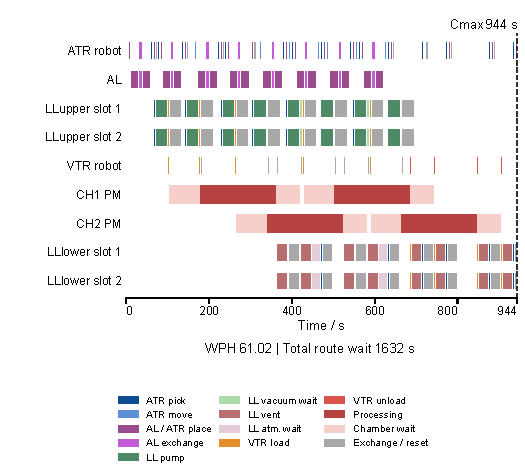
\includegraphics[width=\linewidth]{fig_resource_gantt_cleanH10_w16_41_en_nature}
\caption{16-wafer pure $4\times1$ schedule at $H=10$. No cleaning occurs; $C_{\max}=944$~s, WPH is 61.02 wafers/h, and total route wait is 1632~s.}
\label{fig:gantt-cleanH10-41-en}
\end{figure}

\begin{figure}[!t]
\centering
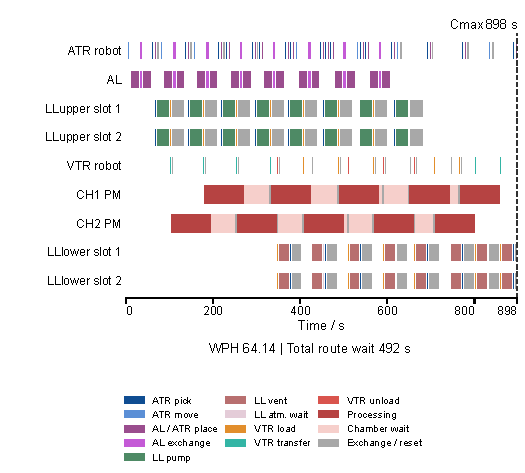
\includegraphics[width=\linewidth]{fig_resource_gantt_cleanH10_w16_22_en_nature}
\caption{16-wafer pure $2\times2$ schedule at $H=10$, without cleaning: $C_{\max}=898$~s, WPH = 64.14 wafers/h. Refinement minimizes total route wait to 492~s at this makespan. Gray denotes 4-s chamber exchanges; pale pink denotes waiting.}
\label{fig:gantt-cleanH10-22-en}
\end{figure}

\begin{figure}[!t]
\centering
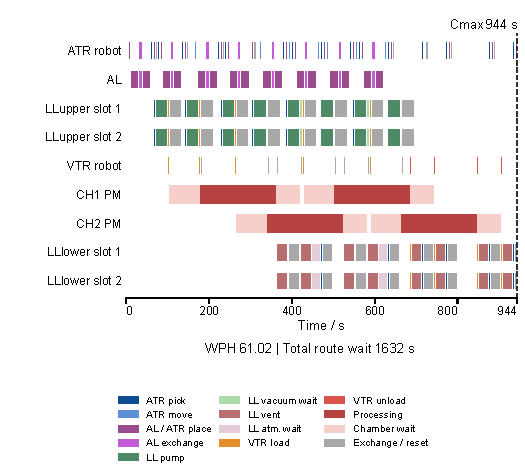
\includegraphics[width=\linewidth]{fig_resource_gantt_cleanH3_w16_41_en_nature}
\caption{16-wafer pure $4\times1$ schedule at $H=3$: $C_{\max}=944$~s, WPH is 61.02 wafers/h, and total route wait is 1632~s.}
\label{fig:gantt-cleanH3-41-en}
\end{figure}

\begin{figure}[!t]
\centering
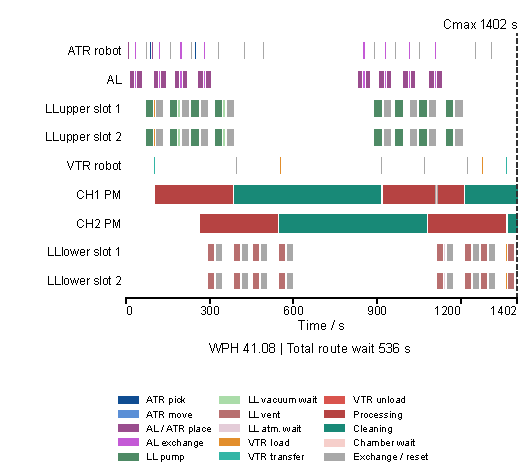
\includegraphics[width=\linewidth]{fig_resource_gantt_cleanH3_w16_22_en_nature}
\caption{16-wafer pure $2\times2$ schedule at $H=3$: two internal and two terminal cleans, $C_{\max}=1402$~s, WPH = 41.08 wafers/h, and total route wait = 536~s. The horizon ends at product return; exchanges and waiting are shown separately.}
\label{fig:gantt-cleanH3-22-en}
\end{figure}

\subsection{Equal-budget refinement of waiting and cadence}

Waiting-time constraints can propagate to manufacturing-system output and control performance \citep{lee2018waiting}. For the same 600-s total budget, the complete two-stage workflow assigns 540~s to the main solve and up to 60~s to refinement, whereas the one-stage control assigns all 600~s to the main solve. Figure~\ref{fig:workflow-en-new} shows that the two-stage workflow reduces total route wait, maximum wait, cadence coefficient of variation, and cadence deviation by 51.91\%, 68.89\%, 39.70\%, and 94.05\%, respectively. All four paired instance differences remain significant after Holm correction, demonstrating that the two-stage workflow markedly improves waiting and cadence quality under the same total budget.

The quadratic-objective control and the complete linear refinement both use the 540+up-to-60-s split. Linear refinement yields a cadence deviation of 22.04, 63.38\% below the quadratic profile's 60.18, and the matched difference remains significant after Holm correction ($p=0.0377$); total route wait, maximum wait, and cadence coefficient of variation are similar overall. The linear objective therefore reduces the measured cadence deviation under the same budget.

\begin{figure}[!htbp]
\centering
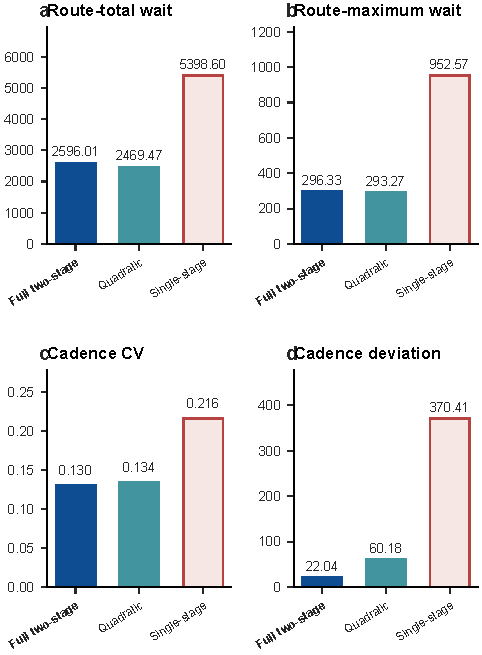
\includegraphics[width=\linewidth]{fig04_workflow_en_nature}
\caption{Final-schedule quality under the same 600-s total budget. a--d, total route wait, maximum route wait, cadence coefficient of variation, and cadence deviation; 1500 runs in total, with observed means labeled above the bars.}
\label{fig:workflow-en-new}
\end{figure}
Table~\ref{tab:refinement-ablation-en} isolates the second stage and refinement objective, complementing the initialization ablation in Table~\ref{tab:spbs-en-new}.

\begin{table*}[!htbp]
\centering\scriptsize
\setlength{\tabcolsep}{3pt}
\caption{Ablation of second-stage refinement and objective form. Each configuration contains 20 instances and 500 runs under a 600-s total budget. Entries are instance-aggregated means; lower is better.}
\label{tab:refinement-ablation-en}
\begin{tabular}{ccccc}
\toprule
Configuration & Total wait (s) & Max. wait (s) & Cadence CV & Deviation (s)\\
\midrule
Full linear refinement & 2596.01 & 296.33 & 0.130 & 22.04\\
Quadratic refinement & 2469.47 & 293.27 & 0.134 & 60.18\\
Without stage two & 5398.60 & 952.57 & 0.216 & 370.41\\
\bottomrule
\end{tabular}
\end{table*}


\subsection{SPBS and structure-aware cut selection}

Table~\ref{tab:spbs-en-new} summarizes the paired SPBS study with 48 instances and ten paired seeds per instance. The timed comparison measures main-solver performance after offline SPBS construction. Relative to the no-start condition, precomputed SPBS increases incumbent availability from 51.67\% to 100\%, a gain of 48.33 percentage points (95\% interval $[34.58,62.29]$). Mean PDI falls from 27473.05 to 20278.78, a decrease of 7194.27 or 26.19\% (95\% interval $[5145.78,9317.61]$). Both paired differences remain significant after Holm correction ($p=2.55\times10^{-5}$ and $p=3.46\times10^{-8}$). Precomputed SPBS therefore improves feasible-schedule availability and primal--dual convergence during the subsequent solve.

\begin{table}[!htbp]
\centering
\scriptsize
\setlength{\tabcolsep}{3pt}
\caption{Effect of precomputed SPBS on time-limited MILP search; construction time is excluded. Each condition contains 48 instances and ten paired seeds per instance, totaling 480 runs.}
\label{tab:spbs-en-new}
\begin{tabular}{cccc}
\toprule
Metric & No start & SPBS & Observed change\\
\midrule
Incumbent rate (\%) & 51.67 & 100.00 & +48.33 points\\
Mean PDI & 27473.05 & 20278.78 & -26.19\%\\
\bottomrule
\end{tabular}
\end{table}

HEM-13D is the most direct learning baseline for the structure-aware cut selector. Both methods share SPBS, training instances, random seeds, candidate limits, hidden dimensions, and a 600-s solve budget, with 500 runs per method. Table~\ref{tab:hem-direct-en} reports this prespecified direct comparison. Relative to HEM-13D, \method{} changes mean PDI from 16823.18 to 16585.70, mean solve time from 219.65 to 218.32~s, mean terminal gap from 127.24\% to 126.01\%, and proven-optimal rate from 62.4\% to 63.2\%. All 500 complete-method runs produce feasible schedules. After aggregating repeats over 20 manufacturing instances, all four paired mean-difference 95\% bootstrap intervals include zero and all Holm-adjusted $p$-values are 1.0. The observed means are close, and the paired tests do not detect significant differences under the common SPBS condition.

\begin{table}[!htbp]
\centering
\scriptsize
\caption{Direct comparison of \method{} and HEM-13D under a common SPBS and budget.}
\label{tab:hem-direct-en}
\begin{tabular}{lrrr}
\toprule
Metric & HEM-13D & \method{} & Observed change\\
\midrule
Mean PDI & 16823.18 & 16585.70 & -1.41\%\\
Mean solution time (s) & 219.65 & 218.32 & -0.61\%\\
Mean terminal gap (\%) & 127.24 & 126.01 & -0.97\%\\
Proven-optimal rate (\%) & 62.4 & 63.2 & +0.80 points\\
\bottomrule
\end{tabular}
\end{table}

The comparison evaluates role-aware representation, sequence decoding, and structural completion jointly under common initialization and solver budgets. It finds no significant performance difference from HEM-13D on the tested instances.

\subsection{Scale, recipe composition, and computational difficulty}

The factorial design contains $4\times5\times3=60$ wafer-count--recipe-composition--process-scale cells with five solver seeds per cell, for 300 runs. Figure~\ref{fig:doe-en-new} shows a sharp transition. All 75 runs at both 8 and 16 wafers prove optimality, with mean PDI values of 28.13 and 1876.54 and mean solution times of 0.34 and 33.86~s. At 24 and 32 wafers, the proven-optimal rates fall to 36\% and 20\%, mean PDI rises to 31155.94 and 32959.89, and mean solution time reaches 408.55 and 433.20~s.

The prespecified PDI factorial model has $R^2=0.998$. Under the $1{:}1$ mixed recipe, the additional interaction coefficients at 24 and 32 wafers are 37729.48 and 40788.63, while the 95\% intervals for the process-scale main effect and all prespecified process-scale interactions include zero. Over the tested 0.9--1.1 process-scale range, computational difficulty is driven primarily by the interaction between batch size and mixed-flow composition, with a comparatively small process-scale effect.

\begin{figure}[!htbp]
\centering
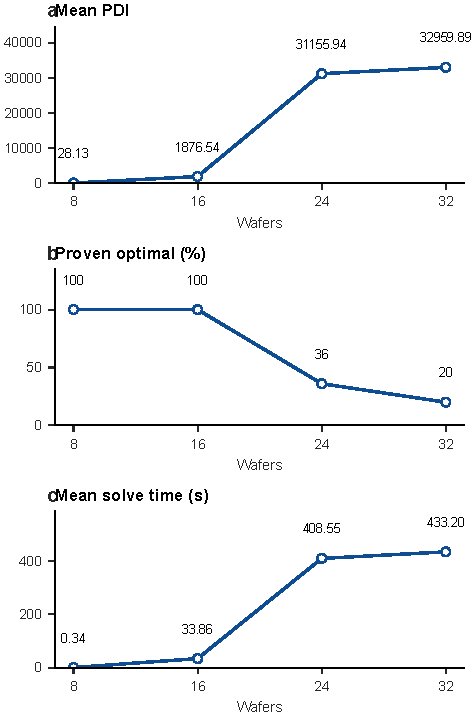
\includegraphics[width=\linewidth]{fig05_doe_en_nature}
\caption{Scale transition in the 300-run factorial experiment. a, mean PDI; b, proven-optimal rate; c, mean solution time. Each wafer count contains 75 runs and observed values are labeled directly.}
\label{fig:doe-en-new}
\end{figure}

\subsection{Operation under parameter perturbations}

Prior CT studies show that cleaning actions and their triggering conditions alter robot-task sequences, cycle time, and wafer delay \citep{yu2020delay,li2022conditioncleaning}. The one-factor sensitivity study therefore covers eight prescribed perturbations of transport, processing, cleaning interval, and vacuum-domain dummy inventory, for 80 runs. Every run returns a solver-checked feasible schedule and 20 runs prove optimality; scenario mean PDI ranges from 28899.41 to 42478.32. A longer cleaning interval gives the lowest mean PDI and slower transport the highest, describing the variation in search performance across the tested parameter settings.

\subsection{Feasible-schedule delivery under distribution shift}

The distribution-shift suite enlarges batches to 40--64 wafers and changes mixed-flow composition, producing 729 runs across all compared methods over nine shifted manufacturing scenarios, including 135 runs of the complete method. This experiment evaluates schedule availability and search performance under changes in scale and composition. All 729 runs return an incumbent that passes SCIP and independent post-solve checks. The shared SPBS--MILP--SCIP chain therefore continues to output a validated resource-action schedule over the tested changes in scale and recipe composition. No run proves optimality. The complete method has mean PDI 73919.15, compared with 73670.99 for default SCIP and 70915.54 for adaptive cut scoring. Feasible-schedule availability is 100\% across this suite, while adaptive cut scoring has the lowest observed mean PDI.

\FloatBarrier

\subsection{Manufacturing-system integration and operational implications}

The framework organizes equipment-cell decisions into configuration input, schedule generation, and event output. MES and process management supply batches, sources, and recipes; equipment configuration supplies capacities, dummy inventory, and cleaning rules. The decision layer coordinates dual-source supply, full-occupancy processing, cleaning, and return and reports timed resource events, makespan, and solver status. The proposed controller interface defines mappings from these records to tool actions and feedback fields for actual completion times, resource states, and frozen actions.

The cleaning grid provides quantitative mode-selection guidance for a given lot. Pure $2\times2$ is preferred for 8 wafers throughout $H=3$--10. For 16 wafers, pure $4\times1$, 1:1 mixed operation, and pure $2\times2$ are preferred at $H=3$, $H=4$, and $H=5$--10, respectively. At $H=4$, mixed operation has only terminal cleaning and yields the shortest makespan of 939~s; at $H\ge5$, pure $2\times2$ can use one complete processing chain per chamber. These comparisons connect batch mode configuration to cleaning organization.

Different components support schedule delivery and timing quality. SPBS achieves 100\% feasible-schedule availability in its experiment, while the equal-budget two-stage workflow significantly reduces waiting and cadence variation. The two learning-based cut selectors have similar average performance with common SPBS, with no statistically significant paired differences. Across all methods, the scale extension delivers feasible schedules in 729 runs with 40--64 wafers, including 135 runs of the complete method. Together, these results connect configuration, material coordination, timing quality, and solver status within an equipment-cell decision process.

\FloatBarrier
\section{Conclusions}

This study develops an operational decision framework for dual-source mixed-flow PECVD rotating-chamber equipment. Product and dummy PWs connect atmospheric-side and vacuum-side logistics. The two-stage MILP jointly represents full-occupancy processing, dummy reuse, periodic cleaning, residency, and shared-resource order and generates complete finite-batch event schedules.

Experiments on three preset modes with prescribed PW layouts and equal cumulative nominal processing time show that lot size and cleaning interval change mode priority through complete-chain segmentation and cleaning position. Pure $2\times2$ is preferred for 8 wafers throughout $H=3$--10. For 16 wafers, pure $4\times1$, 1:1 mixed operation, and pure $2\times2$ are preferred at $H=3$, 4, and 5--10, respectively. For 24 wafers, the corresponding intervals are $H=3$--5, 6, and 7--10. At 16 wafers and $H=6$--10, the pure $2\times2$ optimum is 898~s, 4.87\% below pure $4\times1$. At 24 wafers and $H=7$--10, its feasible upper bound of 1237~s is below both competing optima. Mode selection therefore requires comparison at the relevant lot size and cleaning layout.

Under the same 600-s total budget, the two-stage workflow reduces total route wait, maximum wait, cadence coefficient of variation, and cadence deviation by 51.91\%, 68.89\%, 39.70\%, and 94.05\%, respectively. With precomputed initial schedules, SPBS increases feasible-schedule availability during the timed main solve from 51.67\% to 100\% and reduces mean PDI by 26.19\%. With common SPBS, \method{} and HEM-13D have similar means on all four measures, and paired differences are not significant after multiplicity correction. Across all methods, the 729 distribution-shift runs with 40--64 wafers deliver feasible schedules, including 135 runs of the complete method.

By scheduling dummies as a material flow requiring closed-loop supply, the framework provides a quantitative basis for mode selection, cleaning organization, and equipment-resource coordination. Future work will address rolling scheduling under stochastic arrivals and equipment disturbances and validate controller adaptation and event-feedback integration.

\section*{CRediT authorship contribution statement}
Lincong Wei was responsible for Conceptualization, Methodology, Software,
Validation, Formal analysis, Investigation, Data curation, Visualization,
Writing -- original draft, and Writing -- review and editing. Lizhen Shao was
responsible for Conceptualization, Methodology, Formal analysis, Validation,
Writing -- review and editing, and Project administration. Wei Wang was
responsible for Formal analysis, Investigation, Writing -- review and editing,
and Supervision. All authors reviewed and approved the final manuscript.

\section*{Declaration of competing interest}
The authors declare that they have no known competing financial interests or
personal relationships that could have appeared to influence the work
reported in this paper.

\section*{Data and code availability}
The data, mathematical instances, trained models, and source code supporting
the findings are available from the corresponding author on reasonable
request. 

\section*{Declaration of generative AI and AI-assisted technologies in the manuscript preparation process}
During the preparation of this work, the authors used OpenAI ChatGPT and Codex
to assist with language editing, Chinese--English translation, LaTeX consistency checks, and figure-production code. Research-code assistance is described with the computational methods. After using these tools, the authors reviewed and edited
the content as needed and take full responsibility for the content of the
publication.

\footnotesize
\setlength{\bibsep}{0pt}
\begin{thebibliography}{44}
\expandafter\ifx\csname natexlab\endcsname\relax\def\natexlab#1{#1}\fi
\providecommand{\url}[1]{\texttt{#1}}
\providecommand{\href}[2]{#2}
\providecommand{\path}[1]{#1}
\providecommand{\DOIprefix}{doi:}
\providecommand{\ArXivprefix}{arXiv:}
\providecommand{\URLprefix}{URL: }
\providecommand{\Pubmedprefix}{pmid:}
\providecommand{\doi}[1]{\href{http://dx.doi.org/#1}{\path{#1}}}
\providecommand{\Pubmed}[1]{\href{pmid:#1}{\path{#1}}}
\providecommand{\bibinfo}[2]{#2}
\ifx\xfnm\relax \def\xfnm[#1]{\unskip,\space#1}\fi
%Type = Article
\bibitem[{{Applied Materials}(n.d.)}]{appliedprecisioncvd}
Applied Materials, n.d.
\newblock Producer XP Precision CVD.
\newblock \url{https://www.appliedmaterials.com/us/en/product-library/producer-xp-precision-cvd.html} (accessed 7 September 2026).

\bibitem[{Pan et~al.(2018)Pan, Zhou, Qiao and Wu}]{pan2018survey}
\bibinfo{author}{Pan, C.R.}, \bibinfo{author}{Zhou, M.C.},
  \bibinfo{author}{Qiao, Y.}, \bibinfo{author}{Wu, N.Q.},
  \bibinfo{year}{2018}.
\newblock \bibinfo{title}{Scheduling cluster tools in semiconductor manufacturing:
  Recent advances and challenges}.
\newblock \bibinfo{journal}{IEEE Transactions on Automation Science and Engineering}
  \bibinfo{volume}{15}, \bibinfo{number}{2}, \bibinfo{pages}{586--601}.
\newblock \DOIprefix\doi{10.1109/TASE.2016.2642997}.
%Type = Article

\bibitem[{Gu et~al.(2024)Gu, Wu, Qiao, Zhang and Li}]{gu2024applied}
\bibinfo{author}{Gu, L.}, \bibinfo{author}{Wu, N.},
  \bibinfo{author}{Qiao, Y.}, \bibinfo{author}{Zhang, S.},
  \bibinfo{author}{Li, T.}, \bibinfo{year}{2024}.
\newblock \bibinfo{title}{Scheduling cluster tools with multi-space process
  modules and a multi-finger-arm robot in wafer fabrication subject to wafer
  residency time constraints}.
\newblock \bibinfo{journal}{Applied Sciences} \bibinfo{volume}{14},
  \bibinfo{pages}{9490}.
\newblock \DOIprefix\doi{10.3390/app14209490}.
%Type = Article

\bibitem[{Gu et~al.(2024)Gu, Wu, Qiao and Zhang}]{gu2024multifinger}
\bibinfo{author}{Gu, L.}, \bibinfo{author}{Wu, N.}, \bibinfo{author}{Qiao, Y.},
  \bibinfo{author}{Zhang, S.}, \bibinfo{year}{2024}.
\newblock \bibinfo{title}{Scheduling of {Multi-finger-robotic Cluster Tools}
  with {Multi-space Process Modules}}, in: \bibinfo{booktitle}{2024
  International Conference on Networking, Sensing and Control ({ICNSC})},
  \bibinfo{publisher}{IEEE}.
\newblock \DOIprefix\doi{10.1109/ICNSC62968.2024.10760109}.
%Type = Article

\bibitem[{Li et~al.(2025)Li, Liu, Li and Gao}]{li2025selforganizing}
\bibinfo{author}{Li, Y.}, \bibinfo{author}{Liu, Q.},
  \bibinfo{author}{Li, X.}, \bibinfo{author}{Gao, L.}, \bibinfo{year}{2025}.
\newblock \bibinfo{title}{Manufacturing resource-based self-organizing
  scheduling using multi-agent system and deep reinforcement learning}.
\newblock \bibinfo{journal}{Journal of Manufacturing Systems}
  \bibinfo{volume}{79}, \bibinfo{pages}{179--198}.
\newblock \DOIprefix\doi{10.1016/j.jmsy.2025.01.004}.
%Type = Article

\bibitem[{Zhu et~al.(2025)Zhu, Liu, Yu and Fu}]{zhu2025matrix}
\bibinfo{author}{Zhu, T.}, \bibinfo{author}{Liu, X.},
  \bibinfo{author}{Yu, Y.}, \bibinfo{author}{Fu, L.}, \bibinfo{year}{2025}.
\newblock \bibinfo{title}{Matrix manufacturing system layout and scheduling
  via graph neural network and multi-action deep reinforcement learning}.
\newblock \bibinfo{journal}{Journal of Manufacturing Systems}
  \bibinfo{volume}{82}, \bibinfo{pages}{239--253}.
\newblock \DOIprefix\doi{10.1016/j.jmsy.2025.06.005}.
%Type = Article

\bibitem[{Bhatta and Chang(2025)}]{bhatta2025scaling}
\bibinfo{author}{Bhatta, K.}, \bibinfo{author}{Chang, Q.},
  \bibinfo{year}{2025}.
\newblock \bibinfo{title}{Train small, deploy large: Scaling multi-agent
  reinforcement learning for multi-stage manufacturing lines}.
\newblock \bibinfo{journal}{Journal of Manufacturing Systems}
  \bibinfo{volume}{81}, \bibinfo{pages}{155--168}.
\newblock \DOIprefix\doi{10.1016/j.jmsy.2025.04.017}.
%Type = Article

\bibitem[{Chen et~al.(2024)Chen, Zhang, Wu, Zhang and Wang}]{chen2024idwfs}
\bibinfo{author}{Chen, D.}, \bibinfo{author}{Zhang, J.},
  \bibinfo{author}{Wu, L.}, \bibinfo{author}{Zhang, P.},
  \bibinfo{author}{Wang, M.}, \bibinfo{year}{2024}.
\newblock \bibinfo{title}{Industrial data space application framework for
  semiconductor wafer manufacturing system scheduling}.
\newblock \bibinfo{journal}{Journal of Manufacturing Systems}
  \bibinfo{volume}{77}, \bibinfo{pages}{464--482}.
\newblock \DOIprefix\doi{10.1016/j.jmsy.2024.09.013}.
%Type = Article

\bibitem[{Chen et~al.(2025)Chen, Zhang, Wu, Zhang, Lv, Wang and
  Wang}]{chen2025dgrl}
\bibinfo{author}{Chen, D.}, \bibinfo{author}{Zhang, J.},
  \bibinfo{author}{Wu, L.}, \bibinfo{author}{Zhang, P.},
  \bibinfo{author}{Lv, Y.}, \bibinfo{author}{Wang, J.},
  \bibinfo{author}{Wang, H.}, \bibinfo{year}{2025}.
\newblock \bibinfo{title}{Optimisation method for semiconductor wafer
  manufacturing system scheduling: Reinforcement learning with decision graph
  guiding}.
\newblock \bibinfo{journal}{Journal of Manufacturing Systems}
  \bibinfo{volume}{82}, \bibinfo{pages}{1158--1170}.
\newblock \DOIprefix\doi{10.1016/j.jmsy.2025.08.004}.
%Type = Article

\bibitem[{Kim et~al.(2025)Kim, Kim, Barde and Lee}]{kim2025yieldmakespan}
\bibinfo{author}{Kim, M.G.}, \bibinfo{author}{Kim, H.},
  \bibinfo{author}{Barde, S.}, \bibinfo{author}{Lee, C.H.},
  \bibinfo{year}{2025}.
\newblock \bibinfo{title}{Balancing yield and makespan in wafer fabrication: A
  two-stage data-driven scheduling approach}.
\newblock \bibinfo{journal}{Journal of Manufacturing Systems}
  \bibinfo{volume}{82}, \bibinfo{pages}{874--904}.
\newblock \DOIprefix\doi{10.1016/j.jmsy.2025.07.009}.
%Type = Article

\bibitem[{Lee et~al.(2026)Lee, Lee, Kim, Lee and Kim}]{lee2026quality}
\bibinfo{author}{Lee, S.W.}, \bibinfo{author}{Lee, D.H.},
  \bibinfo{author}{Kim, M.C.}, \bibinfo{author}{Lee, S.Y.},
  \bibinfo{author}{Kim, H.J.}, \bibinfo{year}{2026}.
\newblock \bibinfo{title}{A decomposition-based optimization method for
  parallel machine scheduling under quality uncertainty in wafer manufacturing}.
\newblock \bibinfo{journal}{Journal of Manufacturing Systems}
  \bibinfo{volume}{85}, \bibinfo{pages}{386--401}.
\newblock \DOIprefix\doi{10.1016/j.jmsy.2026.02.002}.
%Type = Article

\bibitem[{Perkinson et~al.(1994)Perkinson, McLarty, Gyurcsik and
  Cavin}]{perkinson1994throughput}
\bibinfo{author}{Perkinson, T.L.}, \bibinfo{author}{McLarty, P.K.},
  \bibinfo{author}{Gyurcsik, R.S.}, \bibinfo{author}{Cavin, R.K.},
  \bibinfo{year}{1994}.
\newblock \bibinfo{title}{Single-wafer cluster tool performance: An analysis
  of throughput}.
\newblock \bibinfo{journal}{IEEE Transactions on Semiconductor Manufacturing}
  \bibinfo{volume}{7}, \bibinfo{pages}{369--373}.
\newblock \DOIprefix\doi{10.1109/66.311340}.
%Type = Article

\bibitem[{Rostami and Hamidzadeh(2002)}]{rostami2002optimal}
\bibinfo{author}{Rostami, S.}, \bibinfo{author}{Hamidzadeh, B.},
  \bibinfo{year}{2002}.
\newblock \bibinfo{title}{Optimal scheduling techniques for cluster tools
  with process-module and transport-module residency constraints}.
\newblock \bibinfo{journal}{IEEE Transactions on Semiconductor Manufacturing}
  \bibinfo{volume}{15}, \bibinfo{pages}{341--349}.
\newblock \DOIprefix\doi{10.1109/TSM.2002.801379}.
%Type = Article

\bibitem[{Wu and Zhou(2010)}]{wu2010closedform}
\bibinfo{author}{Wu, N.Q.}, \bibinfo{author}{Zhou, M.C.},
  \bibinfo{year}{2010}.
\newblock \bibinfo{title}{A closed-form solution for schedulability and
  optimal scheduling of dual-arm cluster tools with wafer residency time
  constraint based on steady schedule analysis}.
\newblock \bibinfo{journal}{IEEE Transactions on Automation Science and
  Engineering} \bibinfo{volume}{7}, \bibinfo{pages}{303--315}.
\newblock \DOIprefix\doi{10.1109/TASE.2008.2008633}.
%Type = Article

\bibitem[{Qiao et~al.(2012)Qiao, Wu and Zhou}]{qiao2012sojourn}
\bibinfo{author}{Qiao, Y.}, \bibinfo{author}{Wu, N.Q.},
  \bibinfo{author}{Zhou, M.C.}, \bibinfo{year}{2012}.
\newblock \bibinfo{title}{Petri net modeling and wafer sojourn time analysis
  of single-arm cluster tools with residency time constraints and activity
  time variation}.
\newblock \bibinfo{journal}{IEEE Transactions on Semiconductor Manufacturing}
  \bibinfo{volume}{25}, \bibinfo{pages}{432--446}.
\newblock \DOIprefix\doi{10.1109/TSM.2012.2199338}.
%Type = Article

\bibitem[{Qiao et~al.(2014)Qiao, Wu and Zhou}]{qiao2014revisiting}
\bibinfo{author}{Qiao, Y.}, \bibinfo{author}{Wu, N.},
  \bibinfo{author}{Zhou, M.C.}, \bibinfo{year}{2014}.
\newblock \bibinfo{title}{Scheduling of dual-arm cluster tools with wafer
  revisiting and residency time constraints}.
\newblock \bibinfo{journal}{IEEE Transactions on Industrial Informatics}
  \bibinfo{volume}{10}, \bibinfo{pages}{286--300}.
\newblock \DOIprefix\doi{10.1109/TII.2013.2272702}.
%Type = Article

\bibitem[{Wang et~al.(2020)Wang, Hu, Pan, Zhou and Li}]{wang2020multiple}
\bibinfo{author}{Wang, J.}, \bibinfo{author}{Hu, H.},
  \bibinfo{author}{Pan, C.}, \bibinfo{author}{Zhou, Y.},
  \bibinfo{author}{Li, L.}, \bibinfo{year}{2020}.
\newblock \bibinfo{title}{Scheduling dual-arm cluster tools with multiple
  wafer types and residency time constraints}.
\newblock \bibinfo{journal}{IEEE/CAA Journal of Automatica Sinica}
  \bibinfo{volume}{7}, \bibinfo{pages}{776--789}.
\newblock \DOIprefix\doi{10.1109/JAS.2020.1003150}.
%Type = Article

\bibitem[{Wang et~al.(2025)Wang, Liu, Zhou and
  Abusorrah}]{wang2025virtualcell}
\bibinfo{author}{Wang, J.}, \bibinfo{author}{Liu, C.},
  \bibinfo{author}{Zhou, M.C.}, \bibinfo{author}{Abusorrah, A.},
  \bibinfo{year}{2025}.
\newblock \bibinfo{title}{Virtual cell-based scheduling approach to
  single-robotic-arm cluster tools subject to wafer residency time
  constraints}.
\newblock \bibinfo{journal}{IEEE Transactions on Automation Science and
  Engineering} \bibinfo{volume}{22}, \bibinfo{pages}{240--251}.
\newblock \DOIprefix\doi{10.1109/TASE.2024.3349380}.
%Type = Article

\bibitem[{Yang et~al.(2025)Yang, Li, Zhen, Zhang and Wu}]{yang2025miptwowafers}
\bibinfo{author}{Yang, F.}, \bibinfo{author}{Li, C.}, \bibinfo{author}{Zhen,
  L.}, \bibinfo{author}{Zhang, C.}, \bibinfo{author}{Wu, N.},
  \bibinfo{year}{2025}.
\newblock \bibinfo{title}{Scheduling residency time-constrained single-armed
  cluster tools with two-wafer types via mixed integer programming model}.
\newblock \bibinfo{journal}{Expert Systems with Applications}
  \bibinfo{volume}{288}, \bibinfo{pages}{128209}.
\newblock \DOIprefix\doi{10.1016/j.eswa.2025.128209}.
%Type = Article

\bibitem[{Kim et~al.(2013)Kim, Kim, Lee and Lee}]{kim2013cleaning}
\bibinfo{author}{Kim, H.}, \bibinfo{author}{Kim, H.J.},
  \bibinfo{author}{Lee, J.H.}, \bibinfo{author}{Lee, T.E.},
  \bibinfo{year}{2013}.
\newblock \bibinfo{title}{Scheduling dual-armed cluster tools with cleaning
  processes}.
\newblock \bibinfo{journal}{International Journal of Production Research}
  \bibinfo{volume}{51}, \bibinfo{pages}{3671--3687}.
\newblock \DOIprefix\doi{10.1080/00207543.2012.758392}.
%Type = Article

\bibitem[{Yu and Lee(2020)}]{yu2020delay}
\bibinfo{author}{Yu, T.S.}, \bibinfo{author}{Lee, T.E.},
  \bibinfo{year}{2020}.
\newblock \bibinfo{title}{Wafer delay analysis and control of dual-armed
  cluster tools with chamber cleaning operations}.
\newblock \bibinfo{journal}{International Journal of Production Research}
  \bibinfo{volume}{58}, \bibinfo{pages}{434--447}.
\newblock \DOIprefix\doi{10.1080/00207543.2019.1593547}.
%Type = Article

\bibitem[{Qiao et~al.(2022)Qiao, Lu, Li, Zhang, Wu and Liu}]{qiao2022binary}
\bibinfo{author}{Qiao, Y.}, \bibinfo{author}{Lu, Y.}, \bibinfo{author}{Li, J.},
  \bibinfo{author}{Zhang, S.}, \bibinfo{author}{Wu, N.}, \bibinfo{author}{Liu,
  B.}, \bibinfo{year}{2022}.
\newblock \bibinfo{title}{An efficient binary integer programming model for
  residency time-constrained cluster tools with chamber cleaning requirements}.
\newblock \bibinfo{journal}{IEEE Transactions on Automation Science and
  Engineering} \bibinfo{volume}{19}, \bibinfo{pages}{1757--1771}.
\newblock \DOIprefix\doi{10.1109/TASE.2021.3122576}.
%Type = Article

\bibitem[{Li et~al.(2022)Li, Yang and Zhen}]{li2022conditioncleaning}
\bibinfo{author}{Li, C.}, \bibinfo{author}{Yang, F.}, \bibinfo{author}{Zhen,
  L.}, \bibinfo{year}{2022}.
\newblock \bibinfo{title}{Efficient scheduling approaches to time-constrained
  single-armed cluster tools with condition-based chamber cleaning operations}.
\newblock \bibinfo{journal}{International Journal of Production Research}
  \bibinfo{volume}{60}, \bibinfo{pages}{3555--3568}.
\newblock \DOIprefix\doi{10.1080/00207543.2021.1926568}.
%Type = Inproceedings

\bibitem[{Zhu et~al.(2025)Zhu, Yuan, Wang and Hou}]{zhu2025failuredeadlock}
\bibinfo{author}{Zhu, Q.}, \bibinfo{author}{Yuan, J.},
  \bibinfo{author}{Wang, G.}, \bibinfo{author}{Hou, Y.}, \bibinfo{year}{2025}.
\newblock \bibinfo{title}{Scheduling a single-arm two-cluster tool with a
  process module failure subject to wafer residency time constraints}.
\newblock \bibinfo{journal}{IEEE Transactions on Automation Science and
  Engineering} \bibinfo{volume}{22}, \bibinfo{pages}{667--679}.
\newblock \DOIprefix\doi{10.1109/TASE.2023.3275703}.
%Type = Article

\bibitem[{Kim and Kim(2025)}]{kim2025noncyclicdeadlock}
\bibinfo{author}{Kim, D.}, \bibinfo{author}{Kim, H.J.}, \bibinfo{year}{2025}.
\newblock \bibinfo{title}{Noncyclic scheduling of cluster tools using deep
  reinforcement learning}.
\newblock \bibinfo{journal}{IEEE Transactions on Automation Science and
  Engineering} \bibinfo{volume}{22}, \bibinfo{pages}{24009--24023}.
\newblock \DOIprefix\doi{10.1109/TASE.2025.3632534}.
%Type = Article

\bibitem[{Lee et~al.(2018)Lee, Zhao, Li and Papadopoulos}]{lee2018waiting}
\bibinfo{author}{Lee, J.H.}, \bibinfo{author}{Zhao, C.},
  \bibinfo{author}{Li, J.}, \bibinfo{author}{Papadopoulos, C.T.},
  \bibinfo{year}{2018}.
\newblock \bibinfo{title}{Analysis, design, and control of {Bernoulli}
  production lines with waiting time constraints}.
\newblock \bibinfo{journal}{Journal of Manufacturing Systems}
  \bibinfo{volume}{46}, \bibinfo{pages}{208--220}.
\newblock \DOIprefix\doi{10.1016/j.jmsy.2018.01.001}.
%Type = Article

\bibitem[{Kim and Lee(2025)}]{kim2025adaptivecluster}
\bibinfo{author}{Kim, H.J.}, \bibinfo{author}{Lee, J.H.}, \bibinfo{year}{2025}.
\newblock \bibinfo{title}{Scheduling cluster tools for concurrent processing:
  Deep reinforcement learning with adaptive search}.
\newblock \bibinfo{journal}{IEEE Transactions on Automation Science and
  Engineering} \bibinfo{volume}{22}, \bibinfo{pages}{3783--3796}.
\newblock \DOIprefix\doi{10.1109/TASE.2024.3399818}.
%Type = Article

\bibitem[{Hong et~al.(2026)Hong, Hsu and Chen}]{hong2026ddpgct}
\bibinfo{author}{Hong, T.Y.}, \bibinfo{author}{Hsu, C.Y.},
  \bibinfo{author}{Chen, C.L.}, \bibinfo{year}{2026}.
\newblock \bibinfo{title}{Simulation-based deep reinforcement learning for
  process time optimization in semiconductor cluster tool and an empirical
  study}.
\newblock \bibinfo{journal}{Computers \& Industrial Engineering}
  \bibinfo{volume}{211}, \bibinfo{pages}{111698}.
\newblock \DOIprefix\doi{10.1016/j.cie.2025.111698}.
%Type = Inproceedings

\bibitem[{Tang et~al.(2020)Tang, Agrawal and Faenza}]{tang2020cut}
\bibinfo{author}{Tang, Y.}, \bibinfo{author}{Agrawal, S.},
  \bibinfo{author}{Faenza, Y.}, \bibinfo{year}{2020}.
\newblock \bibinfo{title}{Reinforcement learning for integer programming:
  Learning to cut}, in: \bibinfo{booktitle}{Proceedings of the 37th
  International Conference on Machine Learning}, \bibinfo{publisher}{PMLR}. pp.
  \bibinfo{pages}{9367--9376}.
\newblock \URLprefix \url{https://proceedings.mlr.press/v119/tang20a.html}.
%Type = Article

\bibitem[{Huang et~al.(2022)Huang, Wang, Liu, Zhen, Zhang, Yuan, Hao, Yu and
  Wang}]{huang2022cutranking}
\bibinfo{author}{Huang, Z.}, \bibinfo{author}{Wang, K.}, \bibinfo{author}{Liu,
  F.}, \bibinfo{author}{Zhen, H.L.}, \bibinfo{author}{Zhang, W.},
  \bibinfo{author}{Yuan, M.}, \bibinfo{author}{Hao, J.}, \bibinfo{author}{Yu,
  Y.}, \bibinfo{author}{Wang, J.}, \bibinfo{year}{2022}.
\newblock \bibinfo{title}{Learning to select cuts for efficient mixed-integer
  programming}.
\newblock \bibinfo{journal}{Pattern Recognition} \bibinfo{volume}{123},
  \bibinfo{pages}{108353}.
\newblock \DOIprefix\doi{10.1016/j.patcog.2021.108353}.
%Type = Inproceedings

\bibitem[{Paulus et~al.(2022)Paulus, Zarpellon, Krause, Charlin and
  Maddison}]{paulus2022looking}
\bibinfo{author}{Paulus, M.B.}, \bibinfo{author}{Zarpellon, G.},
  \bibinfo{author}{Krause, A.}, \bibinfo{author}{Charlin, L.},
  \bibinfo{author}{Maddison, C.}, \bibinfo{year}{2022}.
\newblock \bibinfo{title}{Learning to cut by looking ahead: Cutting plane
  selection via imitation learning}, in: \bibinfo{booktitle}{Proceedings of the
  39th International Conference on Machine Learning},
  \bibinfo{publisher}{PMLR}. pp. \bibinfo{pages}{17584--17600}.
\newblock \URLprefix \url{https://proceedings.mlr.press/v162/paulus22a.html}.
%Type = Inproceedings

\bibitem[{Wang et~al.(2023)Wang, Li, Wang, Kuang, Yuan, Zeng, Zhang and
  Wu}]{wang2023hem}
\bibinfo{author}{Wang, Z.}, \bibinfo{author}{Li, X.}, \bibinfo{author}{Wang,
  J.}, \bibinfo{author}{Kuang, Y.}, \bibinfo{author}{Yuan, M.},
  \bibinfo{author}{Zeng, J.}, \bibinfo{author}{Zhang, Y.}, \bibinfo{author}{Wu,
  F.}, \bibinfo{year}{2023}.
\newblock \bibinfo{title}{Learning cut selection for mixed-integer linear
  programming via hierarchical sequence model}, in:
  \bibinfo{booktitle}{Proceedings of the Eleventh International Conference on
  Learning Representations}.
\newblock \URLprefix \url{https://openreview.net/forum?id=Zob4P9bRNcK}.
%Type = Article

\bibitem[{Bloom(1990)}]{bloom1990cim}
Bloom, H., 1990.
\newblock Software and Computer Integrated Manufacturing.
\newblock NISTIR 4468, National Institute of Standards and Technology.
\newblock \DOIprefix\doi{10.6028/NIST.IR.4468}.

\bibitem[{{OPC Foundation}(n.d.)}]{opcfoundationisa95}
OPC Foundation, n.d.
\newblock OPC Unified Architecture---Common Object Model: ISA-95, version 1.00, Section 4.2: ISA-95 Summary.
\newblock \url{https://reference.opcfoundation.org/specs/OPC-10030/4.2} (accessed 6 September 2026).

\bibitem[{{NAURA}(n.d.)}]{naura2026cygnus}
NAURA, n.d.
\newblock Cygnus Optima Prime PECVD System.
\newblock \url{https://www.naura.com/product/details_15_2442.html} (accessed 11 September 2026).

\bibitem[{{Syskey Technology}(n.d.)}]{syskey2026pecvd}
Syskey Technology Co., Ltd., n.d.
\newblock PECVD.
\newblock \url{https://www.syskey.com.tw/?action=product&title=PECVD} (accessed 11 September 2026).

\bibitem[{Achterberg(2009)}]{achterberg2009scip}
\bibinfo{author}{Achterberg, T.}, \bibinfo{year}{2009}.
\newblock \bibinfo{title}{{SCIP}: Solving constraint integer programs}.
\newblock \bibinfo{journal}{Mathematical Programming Computation}
  \bibinfo{volume}{1}, \bibinfo{pages}{1--41}.
\newblock \DOIprefix\doi{10.1007/s12532-008-0001-1}.
%Type = Article

\bibitem[{Bestuzheva et~al.(2023)Bestuzheva, Besan{\c{c}}on, Chen, Chmiela,
  Donkiewicz, van Doornmalen, Eifler, Gaul, Gamrath, Gleixner, Gottwald,
  Graczyk, Halbig, Hoen, Hojny, van~der Hulst, Koch, L{\"u}bbecke, Maher,
  Matter, M{\"u}hmer, M{\"u}ller, Pfetsch, Schl{\"o}sser, Serrano, Shinano,
  Sofranac, Turner, Vigerske, Wegscheider, Wellner, Weninger and
  Witzig}]{bestuzheva2023scip}
\bibinfo{author}{Bestuzheva, K.}, \bibinfo{author}{Besan{\c{c}}on, M.},
  \bibinfo{author}{Chen, W.K.}, \bibinfo{author}{Chmiela, A.},
  \bibinfo{author}{Donkiewicz, T.}, \bibinfo{author}{van Doornmalen, J.},
  \bibinfo{author}{Eifler, L.}, \bibinfo{author}{Gaul, O.},
  \bibinfo{author}{Gamrath, G.}, \bibinfo{author}{Gleixner, A.},
  \bibinfo{author}{Gottwald, L.}, \bibinfo{author}{Graczyk, C.},
  \bibinfo{author}{Halbig, K.}, \bibinfo{author}{Hoen, A.},
  \bibinfo{author}{Hojny, C.}, \bibinfo{author}{van~der Hulst, R.},
  \bibinfo{author}{Koch, T.}, \bibinfo{author}{L{\"u}bbecke, M.E.},
  \bibinfo{author}{Maher, S.J.}, \bibinfo{author}{Matter, F.},
  \bibinfo{author}{M{\"u}hmer, E.}, \bibinfo{author}{M{\"u}ller, B.},
  \bibinfo{author}{Pfetsch, M.E.}, \bibinfo{author}{Schl{\"o}sser, F.},
  \bibinfo{author}{Serrano, F.}, \bibinfo{author}{Shinano, Y.},
  \bibinfo{author}{Sofranac, B.}, \bibinfo{author}{Turner, M.},
  \bibinfo{author}{Vigerske, S.}, \bibinfo{author}{Wegscheider, F.},
  \bibinfo{author}{Wellner, P.}, \bibinfo{author}{Weninger, D.},
  \bibinfo{author}{Witzig, J.}, \bibinfo{year}{2023}.
\newblock \bibinfo{title}{Enabling research through the {SCIP} optimization
  suite 8.0}.
\newblock \bibinfo{journal}{ACM Transactions on Mathematical Software}
  \bibinfo{volume}{49}, \bibinfo{pages}{22:1--22:21}.
\newblock \DOIprefix\doi{10.1145/3585516}.
%Type = Inproceedings

\bibitem[{Wang et~al.(2024)Wang, Wang, Li, Kuang, Shi, Zhu, Yuan, Zeng, Zhang and Wu}]{wang2024hemset}
Wang, J., Wang, Z., Li, X., Kuang, Y., Shi, Z., Zhu, F., Yuan, M., Zeng, J., Zhang, Y., Wu, F., 2024.
\newblock Learning to Cut via Hierarchical Sequence/Set Model for Efficient Mixed-Integer Programming.
\newblock arXiv:2404.12638.
\newblock \URLprefix \url{https://arxiv.org/abs/2404.12638}.

\bibitem[{Vinyals et~al.(2015)Vinyals, Fortunato and
  Jaitly}]{vinyals2015pointer}
\bibinfo{author}{Vinyals, O.}, \bibinfo{author}{Fortunato, M.},
  \bibinfo{author}{Jaitly, N.}, \bibinfo{year}{2015}.
\newblock \bibinfo{title}{Pointer networks}, in: \bibinfo{booktitle}{Advances
  in Neural Information Processing Systems}, pp. \bibinfo{pages}{2692--2700}.
%Type = Inproceedings

\bibitem[{Choo et~al.(2022)Choo, Kwon, Kim, Jae, Hottung, Tierney and
  Gwon}]{choo2022beam}
\bibinfo{author}{Choo, J.}, \bibinfo{author}{Kwon, Y.D.}, \bibinfo{author}{Kim,
  J.}, \bibinfo{author}{Jae, J.}, \bibinfo{author}{Hottung, A.},
  \bibinfo{author}{Tierney, K.}, \bibinfo{author}{Gwon, Y.},
  \bibinfo{year}{2022}.
\newblock \bibinfo{title}{Simulation-guided beam search for neural
  combinatorial optimization}, in: \bibinfo{booktitle}{Advances in Neural
  Information Processing Systems}.
\newblock \URLprefix
  \url{https://papers.nips.cc/paper_files/paper/2022/hash/39b9b60f0d149eabd1fff2d7c7d5afc4-Abstract-Conference.html},
  \DOIprefix\doi{10.52202/068431-0637}.
%Type = Article

\bibitem[{Nemhauser et~al.(1978)Nemhauser, Wolsey and
  Fisher}]{nemhauser1978analysis}
\bibinfo{author}{Nemhauser, G.L.}, \bibinfo{author}{Wolsey, L.A.},
  \bibinfo{author}{Fisher, M.L.}, \bibinfo{year}{1978}.
\newblock \bibinfo{title}{An analysis of approximations for maximizing
  submodular set functions---i}.
\newblock \bibinfo{journal}{Mathematical Programming} \bibinfo{volume}{14},
  \bibinfo{pages}{265--294}.
\newblock \DOIprefix\doi{10.1007/BF01588971}.
%Type = Article

\bibitem[{Williams(1992)}]{williams1992reinforce}
\bibinfo{author}{Williams, R.J.}, \bibinfo{year}{1992}.
\newblock \bibinfo{title}{Simple statistical gradient-following algorithms for
  connectionist reinforcement learning}.
\newblock \bibinfo{journal}{Machine Learning} \bibinfo{volume}{8},
  \bibinfo{pages}{229--256}.
\newblock \DOIprefix\doi{10.1007/BF00992696}.
%Type = Inproceedings

\bibitem[{Mnih et~al.(2016)Mnih, Badia, Mirza, Graves, Lillicrap, Harley,
  Silver and Kavukcuoglu}]{mnih2016a3c}
\bibinfo{author}{Mnih, V.}, \bibinfo{author}{Badia, A.P.},
  \bibinfo{author}{Mirza, M.}, \bibinfo{author}{Graves, A.},
  \bibinfo{author}{Lillicrap, T.P.}, \bibinfo{author}{Harley, T.},
  \bibinfo{author}{Silver, D.}, \bibinfo{author}{Kavukcuoglu, K.},
  \bibinfo{year}{2016}.
\newblock \bibinfo{title}{Asynchronous methods for deep reinforcement
  learning}, in: \bibinfo{booktitle}{Proceedings of the 33rd International
  Conference on Machine Learning}, \bibinfo{publisher}{PMLR}. pp.
  \bibinfo{pages}{1928--1937}.
\newblock \URLprefix \url{https://proceedings.mlr.press/v48/mniha16.html}.

\end{thebibliography}

\end{document}
